\documentclass[aspectratio=1610]{beamer}

\usepackage[T1]{fontenc}
\usepackage{amsmath}
\usepackage{enumitem}
\usepackage{pgfplots}
\usepackage{subcaption}
\usepackage{tikz}
\usepackage{colortbl}  % For coloring table rows
\usepackage{array}     % For array package
\usepackage{xcolor}    % For custom colors

% Define custom colors
\definecolor{rowcolor1}{rgb}{0.9, 0.9, 1}  % Light blue
\definecolor{rowcolor2}{rgb}{1, 0.9, 0.9}  % Light red
\pgfplotsset{compat=1.18}

\usetheme{Boadilla}
\setbeamertemplate{navigation symbols}{}
\setbeamercolor{frametitle}{bg=blue, fg=white}
\setbeamertemplate{footline}[frame number]

\title[Fourier Transform]{Fourier Transform}
\subtitle{Decoding the Hidden Language of Signals}
\author{Md junaid ahmmad, Gourove Roy, Sadrul Islam Faysal}
\date{\today}

\begin{document}

\begin{frame}
    \titlepage
\end{frame}

\begin{frame}{Table Of Content}
    \begin{center}
        \vspace{0.5cm}
        \begin{itemize}[]
            \item[\textcolor{blue}{1.}] The Smoothie Analogy
                \begin{itemize}
                    \item From Smoothie to Recipe
                    \item Using Filters
                \end{itemize}
            \vspace{0.3cm}
            
            \item[\textcolor{blue}{2.}] From Smoothies to Signals
                \begin{itemize}
                    \item Drawing the Parallel
                    \item Understanding the Transformation
                \end{itemize}
            \vspace{0.3cm}
            
            \item[\textcolor{blue}{3.}] Building with Fourier Components
                \begin{itemize}
                    \item Component Signals
                    \item Frequency Analysis
                \end{itemize}
            \vspace{0.3cm}
            
            \item[\textcolor{blue}{4.}] Understanding Sine and Cosine
                \begin{itemize}
                    \item Why Both Are Needed
                    \item Complete Representation
                \end{itemize}
        \end{itemize}
    \end{center}
\end{frame}

\begin{frame}{The Smoothie Analogy}
    \begin{center}
        \vspace{0.3cm}
        {\Large{Given a \textcolor{red}{Smoothie} , lets find its \textcolor{red}{Recipe}}}
        
        \vspace{0.6cm}
        \begin{tikzpicture}
            \only<1-2>{
                \node (smoothie) at (-3,0) {
\includegraphics[width=0.4\textwidth]{smoothie.jpeg}};
            }
            
            \only<2>{
                \draw[->, thick, blue!70, line width=2pt] (0,0) -- (2,0);
                \node[above] at (1,0.3) {\textcolor{blue}{Analysis}};
            }
            
            \only<2>{
                \node (recipe) at (5,0) {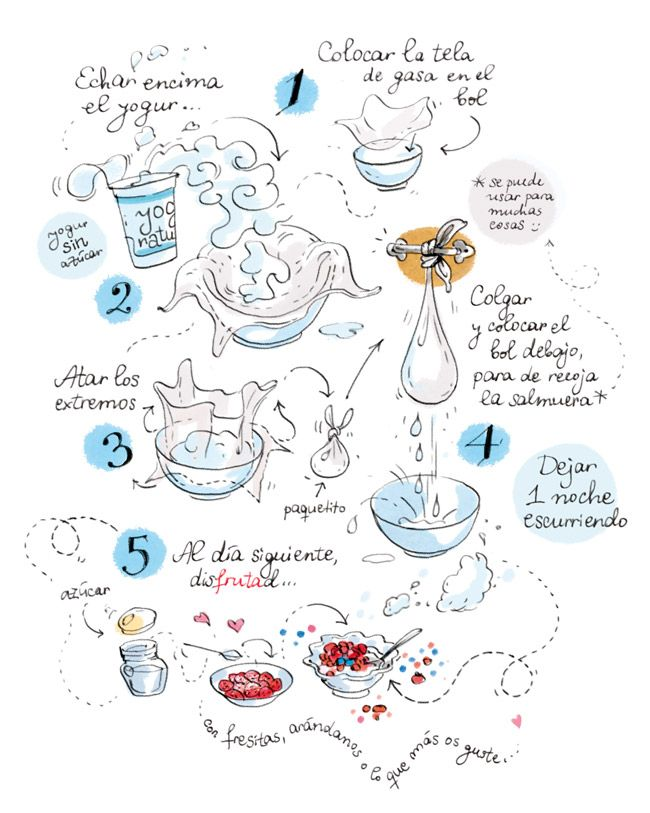
\includegraphics[width=0.4\textwidth]{recipe.jpeg}};
            }
        \end{tikzpicture}
    \end{center}
\end{frame}
\begin{frame}{How Can We Do That?}
    \begin{center}
        \vspace{0.1cm}
        {\Large Extracting the \textcolor{red}{recipe} using \textcolor{red}{filters}}
        \vspace{0.7cm}
        
        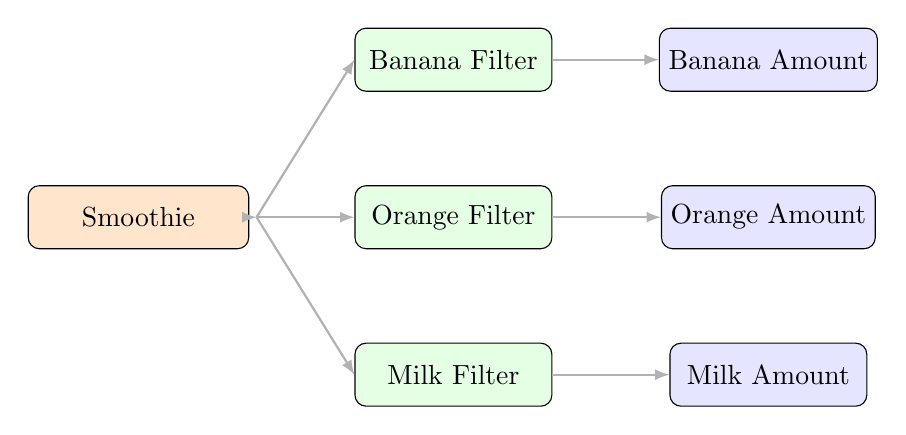
\begin{tikzpicture}[
            box/.style={draw, rounded corners, minimum width=2.5cm, minimum height=0.8cm},
            arrow/.style={->, thick, >=latex, draw=gray!60}
        ]
            % Smoothie on left
            \node[box, fill=orange!20, minimum width=2.8cm] (smoothie) at (-4,0) {Smoothie};
            
            % Filters in middle
            \node[box, fill=green!10] (banana) at (0,2) {Banana Filter};
            \node[box, fill=green!10] (orange) at (0,0) {Orange Filter};
            \node[box, fill=green!10] (milk) at (0,-2) {Milk Filter};
            
            % Amounts on right
            \node[box, fill=blue!10] (bamount) at (4,2) {Banana Amount};
            \node[box, fill=blue!10] (oamount) at (4,0) {Orange Amount};
            \node[box, fill=blue!10] (mamount) at (4,-2) {Milk Amount};
            
            % Connecting arrows from same point
            \coordinate (split) at (-2.5,0);
            \draw[arrow] (smoothie.east) -- (split);
            \draw[arrow] (split) -- (banana.west);
            \draw[arrow] (split) -- (orange.west);
            \draw[arrow] (split) -- (milk.west);
            
            \draw[arrow] (banana) -- (bamount);
            \draw[arrow] (orange) -- (oamount);
            \draw[arrow] (milk) -- (mamount);
            
        \end{tikzpicture}
    \end{center}
\end{frame}


\begin{frame}{From Smoothies to Signals}
    \begin{center}
        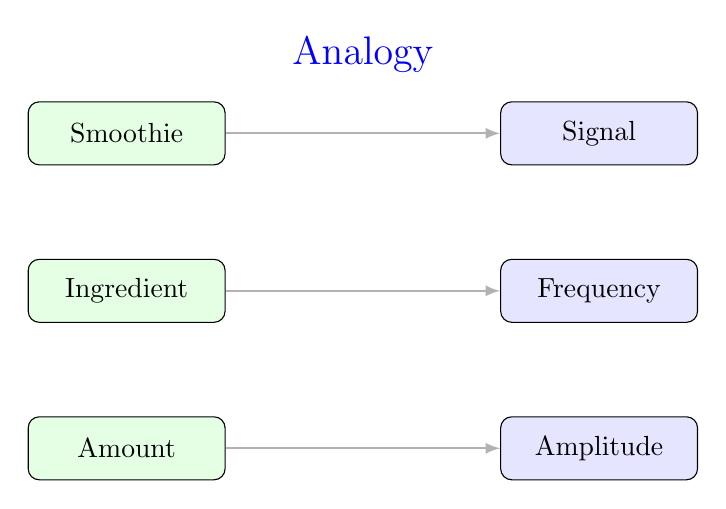
\begin{tikzpicture}[
            box/.style={draw, rounded corners, minimum width=2.5cm, minimum height=0.8cm},
            arrow/.style={->, thick, >=latex, draw=gray!60},
            label/.style={font=\Large}
        ]
            % Title
            \node[label] at (0,3) {\textcolor{blue}{Analogy}};
            
            % Left column - Smoothie concepts
            \node[box, fill=green!10] (smoothie) at (-3,2) {Smoothie};
            \node[box, fill=green!10] (ingredient) at (-3,0) {Ingredient};
            \node[box, fill=green!10] (amount) at (-3,-2) {Amount};
            
            % Right column - Signal concepts
            \node[box, fill=blue!10] (signal) at (3,2) {Signal};
            \node[box, fill=blue!10] (frequency) at (3,0) {Frequency};
            \node[box, fill=blue!10] (amplitude) at (3,-2) {Amplitude};
            
            % Connect related concepts with centered arrows
            \draw[arrow] (smoothie.east) -- (signal.west);
            \draw[arrow] (ingredient.east) -- (frequency.west);
            \draw[arrow] (amount.east) -- (amplitude.west);      
        \end{tikzpicture}
    \end{center}
    \Large{And the whole \textcolor{red}{transformation} process is identical to \textcolor{red}{Fourier transform}. }
\end{frame}


\begin{frame}{Building a Signal: Fourier Components}
    \begin{tikzpicture}
        % Left plot (Component signals)
        \begin{scope}[shift={(-3,0)}, scale=0.9]
            % Grid and axes
            \draw[gray!20, step=1] (-0.5,-2) grid (7,2);
            \draw[thick, ->] (-0.5,0) -- (7,0) node[below] {Time};
            \draw[thick, ->] (0,-2) -- (0,2) node[left] {};
            \node[above] at (3.5, 2.5) {\textbf{Components}};
            
            \only<1>{
                \draw[blue, thick, domain=0:6.5, samples=100] plot (\x, {sin(\x r)});
                \draw[blue, thick] (5.5,1) node {$f_1 = 1$ Hz};
            }
            \only<2>{
                \draw[blue!30, thick, domain=0:6.5, samples=100] plot (\x, {sin(\x r)});
                \draw[blue, thick, domain=0:6.5, samples=100] plot (\x, {0.5*sin(2*\x r)});
                \draw[blue, thick] (5.5,1) node {$f_2 = 2$ Hz};
            }
            \only<3>{
                \draw[blue!30, thick, domain=0:6.5, samples=100] plot (\x, {sin(\x r)});
                \draw[blue!30, thick, domain=0:6.5, samples=100] plot (\x, {0.5*sin(2*\x r)});
                \draw[blue, thick, domain=0:6.5, samples=100] plot (\x, {0.3*sin(3*\x r)});
                \draw[blue, thick] (5.5,1) node {$f_3 = 3$ Hz};
            }
            \only<4>{
                \draw[blue!30, thick, domain=0:6.5, samples=100] plot (\x, {sin(\x r)});
                \draw[blue!30, thick, domain=0:6.5, samples=100] plot (\x, {0.5*sin(2*\x r)});
                \draw[blue!30, thick, domain=0:6.5, samples=100] plot (\x, {0.3*sin(3*\x r)});
                \draw[blue, thick, domain=0:6.5, samples=100] plot (\x, {0.2*sin(4*\x r)});
                \draw[blue, thick] (5.5,1) node {$f_4 = 4$ Hz};
            }
            \only<5>{
                \draw[blue!30, thick, domain=0:6.5, samples=100] plot (\x, {sin(\x r)});
                \draw[blue!30, thick, domain=0:6.5, samples=100] plot (\x, {0.5*sin(2*\x r)});
                \draw[blue!30, thick, domain=0:6.5, samples=100] plot (\x, {0.3*sin(3*\x r)});
                \draw[blue!30, thick, domain=0:6.5, samples=100] plot (\x, {0.2*sin(4*\x r)});
                \draw[blue, thick, domain=0:6.5, samples=100] plot (\x, {0.1*sin(5*\x r)});
                \draw[blue, thick] (5.5,1) node {$f_5 = 5$ Hz};
            }
        \end{scope}

        % Right plot (Combined signal)
        \begin{scope}[shift={(4.5,0)}, scale=0.9]
            \draw[gray!20, step=1] (-0.5,-2) grid (7,2);
            \draw[thick, ->] (-0.5,0) -- (7,0) node[below] {Time};
            \draw[thick, ->] (0,-2) -- (0,2) node[left] {};
            \node[above] at (3.5, 2.5) {\textbf{Combined Signal}};
            
            % Combined signals
            \only<1>{\draw[red, thick, domain=0:6.5, samples=100] 
                plot (\x, {sin(\x r)});}
            \only<2>{\draw[red, thick, domain=0:6.5, samples=100] 
                plot (\x, {sin(\x r) + 0.5*sin(2*\x r)});}
            \only<3>{\draw[red, thick, domain=0:6.5, samples=100] 
                plot (\x, {sin(\x r) + 0.5*sin(2*\x r) + 0.3*sin(3*\x r)});}
            \only<4>{\draw[red, thick, domain=0:6.5, samples=100] 
                plot (\x, {sin(\x r) + 0.5*sin(2*\x r) + 0.3*sin(3*\x r) + 0.2*sin(4*\x r)});}
            \only<5>{\draw[red, thick, domain=0:6.5, samples=100] 
                plot (\x, {sin(\x r) + 0.5*sin(2*\x r) + 0.3*sin(3*\x r) + 0.2*sin(4*\x r) + 0.1*sin(5*\x r)});}
        \end{scope}

        % Explanatory text
        \node[text width=12cm] at (4,-3) {
            \only<1>{Starting with the fundamental frequency}
            \only<2>{Adding the second harmonic}
            \only<3>{Adding the third harmonic}
            \only<4>{Adding the fourth harmonic}
            \only<5>{Final signal with five components}
        };
    \end{tikzpicture}
\end{frame}

\begin{frame}{Fourier Transform Analysis}
    \begin{center}
        \hspace{-1cm}
        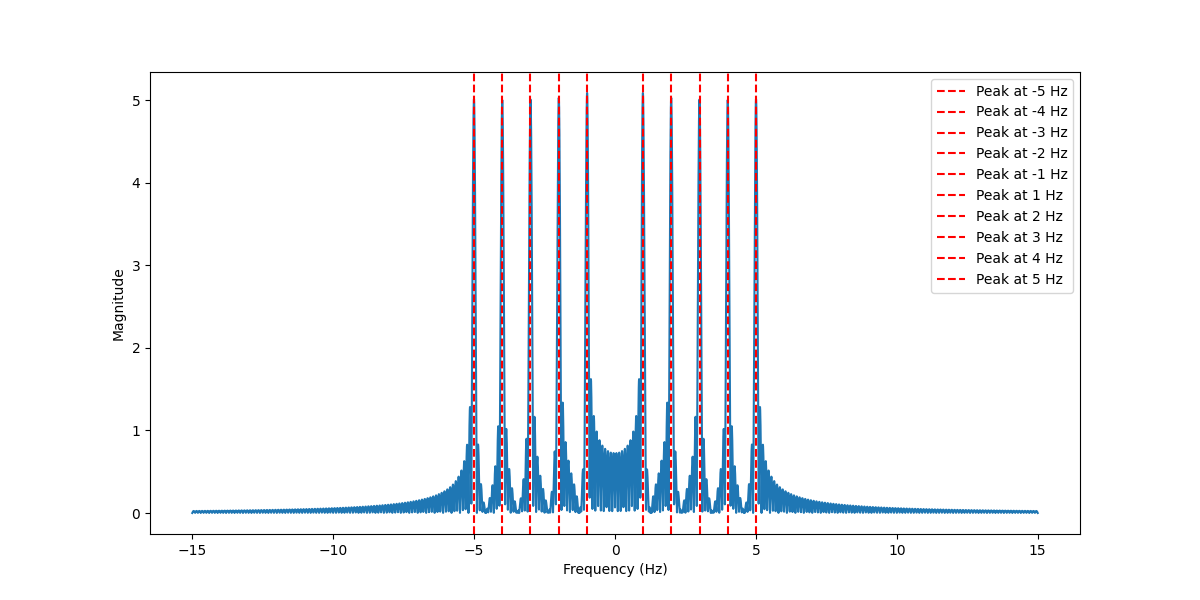
\includegraphics[width=1.1\textwidth]{freq_spectrum.png}
    \end{center}
\end{frame}

\begin{frame}{How Fourier Transform Detects Frequencies}
    \begin{center}
        \vspace{0.3cm}
        \begin{tikzpicture}[scale=1.2]
            \draw[->] (-4,0) -- (4,0) node[right] {\small Time};
            \draw[->] (0,-1.5) -- (0,1.5) node[above] {\small Amplitude};
            
            \only<1-2> {
                \draw[thick, blue, domain=-4:4, samples=100] 
                    plot (\x, {sin(360 * \x / 8)}); 
                \draw[blue, thick] (4.5,1) node {$f_1 = 0.125$ Hz};
            }
            
            \only<2> {
                \draw[thick, red, domain=-4:4, samples=100, dashed] 
                    plot (\x, {sin(360 * \x / 5)}); 
                \draw[red, thick] (4.5,0.5) node {$f_2 = 0.500$ Hz};
            }
            
            \only<3> {
                \fill[purple!20, opacity=0.5] 
                    plot[domain=-4:4, samples=100] 
                    (\x, {sin(360 * \x / 8) * sin(360 * \x / 5)}) -- 
                    (4,0) -- (-4,0) -- cycle;
                \draw[thick, purple, domain=-4:4, samples=100] 
                    plot (\x, {sin(360 * \x / 8) * sin(360 * \x / 5)});
                \node[align=center, below=0.8cm, text=purple] at (0, -1) 
                    {\textbf{Area under curve = 0}};
            }
            
            \only<4> {
                \draw[thick, blue, domain=-4:4, samples=100] 
                    plot (\x, {sin(360 * \x / 8)}); 
                \draw[thick, red, domain=-4:4, samples=100,dashed] 
                    plot (\x, {sin(360 * \x / 8)}); 
                \draw[blue, thick] (4.5,1) node {$f_1 = 0.125$ Hz};
                \draw[red, thick] (4.5,0.5) node {$f_1 = 0.125$ Hz};
            }
            
            \only<5> {
                \fill[purple!20, opacity=0.5] 
                    plot[domain=-4:4, samples=100] 
                    (\x, {sin(360 * \x / 8) * sin(360 * \x / 8)}) -- 
                    (4,0) -- (-4,0) -- cycle;
                \draw[thick, purple, domain=-4:4, samples=100] 
                    plot (\x, {sin(360 * \x / 8) * sin(360 * \x / 8)});
                \node[align=center, below=0.8cm, text=purple] at (0, -1) 
                    {\textbf{Area under curve > 0 (Correlation)}};
            }
        \end{tikzpicture}
    \end{center}
\end{frame}

\begin{frame}{Frequency Domain Representation}
    \begin{center}
        \vspace{0.3cm}
        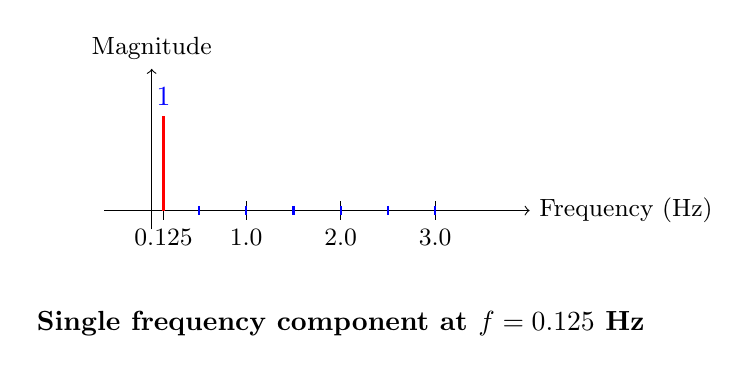
\begin{tikzpicture}[scale=1.2]
            \draw[->] (-0.5,0) -- (4,0) node[right] {\small Frequency (Hz)};
            \draw[->] (0,-0.2) -- (0,1.5) node[above] {\small Magnitude};
            
            \foreach \x/\xtext in {0.125/0.125, 1/1.0, 2/2.0, 3/3.0}
                \draw (\x,0.1) -- (\x,-0.1) node[below] {\small \xtext};
            
            \draw[thick, red] (0.125,0) -- (0.125,1);
            \draw[thick, blue] (0.125,1) -- (0.125,1) node[above] {1};
            
            \foreach \x in {0.5,1,1.5,2,2.5,3}
                \draw[thick, blue] (\x,0.05) -- (\x,-0.05);
                
            \node[align=center] at (2,-1.2) 
                {\textbf{Single frequency component at $f=0.125$ Hz}};
        \end{tikzpicture}
    \end{center}
\end{frame}

\begin{frame}{Why We Need Both Sine and Cosine Terms}
    \begin{center}
        \vspace{0.3cm}
        \begin{tikzpicture}[scale=1.2]
            \draw[->] (-4,0) -- (4,0) node[right] {\small Time};
            \draw[->] (0,-1.5) -- (0,1.5) node[above] {\small Amplitude};
            
            \only<1,2,4>{
                \draw[thick, blue, domain=-4:4, samples=100] 
                    plot (\x, {cos(360 * \x / 8)}); 
                \draw[blue, thick] (4.5,1) node {Target: $\cos(2\pi t)$};
            }
            
            \only<2>{
                \draw[thick, red, domain=-4:4, samples=100, opacity=0.5] 
                    plot (\x, {sin(360 * \x / 8)}); 
                \draw[red, thick] (4.5,0.5) node {Attempt: $\sin(2\pi t)$};
            }

            \only<3> {
                \fill[purple!20, opacity=0.5] 
                    plot[domain=-4:4, samples=1000] 
                    (\x, {cos(360 * \x /8) * sin(360 * \x/8 )}) -- 
                    (4,0) -- (-4,0) -- cycle;
                \draw[thick, purple, domain=-4:4, samples=1000] 
                    plot (\x, {cos(360 * \x /8) * sin(360 * \x/8 )});
                \node[align=center, below=0.8cm, text=purple] at (0, -1) 
                    {\textbf{Area under curve = 0}};
            }
            
            \only<4>{
                \draw[thick, red, domain=-4:4, samples=100, opacity=0.5] 
                    plot (\x, {sin(360 * \x / 8)});
                \draw[thick, blue, domain=-4:4, samples=100, opacity=0.5] 
                    plot (\x, {0.5*sin(720 * \x / 8)});
                \draw[thick, green, domain=-4:4, samples=100, opacity=0.5] 
                    plot (\x, {0.25*sin(1080 * \x / 8)});
                \node[align=center] at (0,-2) 
                    {\textbf{Cannot match cosine with}\\
                     \textbf{any combination of sines}};
            }
            
            \only<5>{
                \draw[thick, blue, domain=-4:4, samples=100, opacity=0.8] 
                    plot (\x, {cos(360 * \x/8 )}); 
                \draw[thick, red, domain=-4:4, samples=100,dashed, opacity=1] 
                    plot (\x, {cos(360 * \x/8 )}); 
                \draw[blue, thick] (4.5,1) node {Target: $\cos(2\pi t)$};
                \draw[red, thick] (4.5,0.5) node {Attempt: $\cos(2\pi t)$};
                \node[align=center] at (0,-2) 
                    {$f(t) = a_0 + \sum\limits_{n=1}^{\infty} (a_n\cos(2\pi nt) + b_n\sin(2\pi nt))$};
            }
        \end{tikzpicture}
    \end{center}
\end{frame}

\begin{frame}{Why Fourier Transform?}
    \begin{itemize}
        \item<1-> Analyze and simplify complex signals like audio, images, and communication data.
        \item<2-> Break signals into fundamental sine and cosine components.
        \item<3-> Applications in:
        \begin{itemize}
            \item Audio processing (e.g., equalizers, compression).
            \item Medical imaging (e.g., MRIs).
            \item Image compression (e.g., JPEGs).
        \end{itemize}
    \end{itemize}
    \pause
    % \includegraphics[width=0.8\textwidth]{example_signal.png}
\end{frame}

\begin{frame}
\textcolor{green}{\textbf{Fourier transform and it's properties}}
\end{frame}

\begin{frame}
    \frametitle{What is Fourier Transformation?(Recap)}
    The \textcolor{red}{generalized form of the complex Fourier series} is referred to as the Fourier transform.
    It helps to expand the \textcolor{red}{non-periodic} functions and convert them into \textcolor{red}{easy sinusoid} functions.
    \begin{figure}
        \centering
        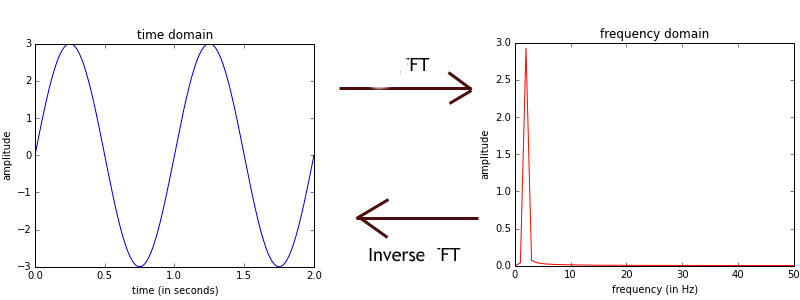
\includegraphics[width=0.9\textwidth]{images/time_freq_domain.png}
        \caption{Fourier Transformation}
    \end{figure}
\end{frame}

\begin{frame}
    \frametitle{Table of Content}
    \begin{itemize}[label=$\star$, itemsep=15pt, parsep=0pt, topsep=10pt]
        \item <1-> Fourier Transform Type
        \item <2-> Forward Fourier Transform
        \item <3-> Inverse Fourier Transform
        \item <4-> Fourier Transform Notation
        \item <5-> Example of Fourier Transform
        \item <6-> Properties of Fourier Transform
        \item <7-> Fourier Transform Table
    \end{itemize}
\end{frame}

\begin{frame}
    \frametitle{Fourier Transform Type}
    There are \textcolor{red}{two} types of Fourier transform i.e., \textcolor{blue}{forward} Fourier transform and \textcolor{blue}{inverse} Fourier transform.\\
    The forward and inverse Fourier transform is used to decompose a function or a signal into its constituent frequencies and times respectively.
\end{frame}

\begin{frame}
    \frametitle{Forward Fourier Transform}
    The forward Fourier transform is a mathematical technique used to transform a \textcolor{blue}{time-domain signal} into its \textcolor{blue}{frequency-domain} representation.
    The forward Fourier transform of a continuous-time signal $x(t)$ is given by
    \begin{equation*}
        X(\omega) = \int_{-\infty}^{\infty} x(t) e^{-j\omega t} dt
    \end{equation*}
    where $X(\omega)$ is the Fourier transform of $x(t)$, $\omega$ is the angular frequency, $j$ is the imaginary unit$(\sqrt{-1})$, and $t$ is the time.
\end{frame}

\begin{frame}
    \frametitle{Inverse Fourier Transform}
    The inverse Fourier transform is the process of \textcolor{blue}{converting a frequency-domain} representation of a signal \textcolor{blue}{back into its time-domain} form.
    The inverse Fourier transform is given by
    \begin{equation*}
        x(t) =\frac{1}{2\pi} \int_{-\infty}^{\infty} X(\omega) e^{j\omega t} d\omega
    \end{equation*}
    where $x(t)$ is the time-domain signal and $X(\omega)$ is the Fourier transform of $x(t)$, $\omega$ is the angular frequency, $j$ is the imaginary unit$(\sqrt{-1})$, and $t$ is the time.
\end{frame}

\begin{frame}
    \frametitle{Fourier Transform Notation}

    \onslide<1->{
    For convenience, we will write the Fourier transform of a signal \(x(t)\) as
    \[
        X(f) = \mathcal{F}\{x(t)\}
    \]
    }

    \onslide<2->{
    and the inverse Fourier transform of \(X(f)\) as
    \[
        x(t) = \mathcal{F}^{-1}\{X(f)\}.
    \]
    }

    \onslide<3->{
    Note that
    \[
        \mathcal{F}^{-1}\{\mathcal{F}\{x(t)\}\} = x(t)
    \]
    at points of continuity of \(x(t)\).
    }
\end{frame}

\begin{frame}
    \frametitle{Example of Fourier Transform}
    \onslide<1->{
        Let $x(t) = rect(t)$ where rect(t) is the rectangular pulse function defined as
        \begin{equation*}
            rect(t) = \begin{cases}
                1 & \text{if } |t| < \frac{1}{2}\\
                0 & \text{otherwise}
            \end{cases}
        \end{equation*}
    }

    \onslide<2->{
        and $sinc(\omega)$ is the sinc function defined as
        \begin{equation*}
            sinc(\omega) = \begin{cases}
                \frac{sin(\omega / 2)}{\omega / 2} & \text{if } \omega \neq 0\\
                1 & \text{if } \omega = 0
            \end{cases}
        \end{equation*}
    }
\end{frame}

\begin{frame}
    \frametitle{Example of Fourier Transform}
    \textcolor{red}{The forward Fourier transform of $rect(t)$ is $sinc(\omega)$} and \textcolor{blue}{the inverse Fourier transform of $sinc(\omega)$ is $rect(t)$.}
    \begin{figure}[ht]
        \centering
        % Rect function
        \begin{subfigure}[b]{0.45\textwidth}
            \centering
            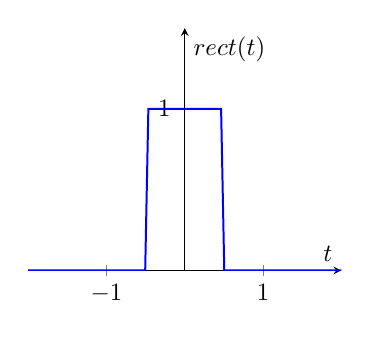
\begin{tikzpicture}[scale=0.9]
                \begin{axis}[
                    domain=-2:2,
                    samples=100,
                    axis lines=middle,
                    xlabel={$t$},
                    ylabel={$rect(t)$},
                    ymin=0, ymax=1.5,
                    xmin=-2, xmax=2,
                    xtick={-1,0,1},
                    ytick={0,1},
                    % grid=major,
                    height=5cm,
                    width=6cm
                ]
                    \addplot[thick,blue] {abs(x) <= 0.5 ? 1 : 0};
                \end{axis}
            \end{tikzpicture}
            \caption{Inverse fourier transform of $sinc(\omega)$}
        \end{subfigure}
        \hfill
        % Sinc function
        \begin{subfigure}[b]{0.45\textwidth}
            \centering
            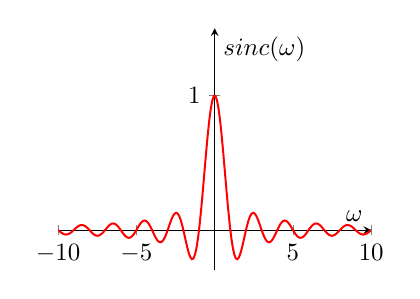
\begin{tikzpicture}[scale=0.9]
                \begin{axis}[
                    domain=-10:10,
                    samples=200,
                    axis lines=middle,
                    xlabel={$\omega$},
                    ylabel={$sinc(\omega)$},
                    ymin=-0.3, ymax=1.5,
                    xmin=-10, xmax=10,
                    xtick={-10,-5,5,10},
                    ytick={1},
                    % grid=major,
                    height=5cm,
                    width=6cm
                ]
                    \addplot[thick,red] {x == 0 ? 1 : sin(deg(pi*x))/(pi*x)};
                \end{axis}
            \end{tikzpicture}
            \caption{forward fourier transform of $rect(t)$}
        \end{subfigure}
    \end{figure}
\end{frame}

\begin{frame}
    \frametitle{Properties of Fourier Transform}
    \begin{itemize}[label=$\star$, itemsep=10pt, parsep=0pt, topsep=8pt]
        \item Linearity
        \item Time Shifting
        \item Time Scaling
        \item Time Reversal
        \item Differentiation
        \item Integration
        \item Convolution
    \end{itemize}
\end{frame}

\begin{frame}
    \frametitle{Properties of Fourier Transform}
    \setbeamercovered{dynamic, transparent = 20} % Enable dimming for unrevealed items

    % The list is shown in overlays where no details are displayed
    \only<1, 7, 11, 15, 19, 22, 25>{
        \begin{itemize}[label=$\star$, itemsep=10pt, parsep=0pt, topsep=8pt]
            \item <1> Linearity
            \item <7> Time Shifting
            \item <11> Time Scaling
            \item <15> Time Reversal
            \item <19> Differentiation
            \item <22> Integration
            \item <25> Convolution
        \end{itemize}
    }

    % Detailed content for Linearity
    \only<2>{
        \begin{block}{Linearity}
            If $x_1(t)$ and $x_2(t)$ are two signals with fourier transform $X_1(\omega)$ and $X_2(\omega)$ respectively, then
            the Fourier transform of a linear combination of the signals is linear:
            \[
            \mathcal{F}\{\textcolor{blue}{a} x_1(t) + \textcolor{red}{b} x_2(t)\} = \textcolor{blue}{a} X_1(\omega) + \textcolor{red}{b} X_2(\omega)
            \]
            where $a$ and $b$ are constants.
        \end{block}
    }

    \only<3>{
        \begin{block}{Linearity}
            Let $x_1(t) = rect(t)$ and $x_2(t) = rect(t)$ be two signals and let $X_1(\omega) = \mathcal{F} \{x_1(t)\} = sinc(\omega)$ and $X_2(\omega) = \mathcal{F} \{x_2(t)\} = sinc(\omega)$ be their fourier transforms respectively.
            \begin{figure}[ht]
                \centering
                % Rect function
                \begin{subfigure}[b]{0.45\textwidth}
                    \centering
                    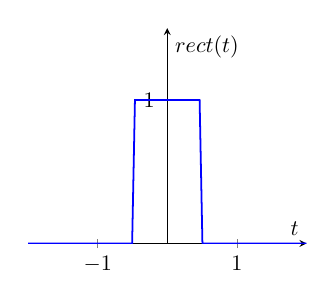
\begin{tikzpicture}[scale=0.8]
                        \begin{axis}[
                            domain=-2:2,
                            samples=100,
                            axis lines=middle,
                            xlabel={$t$},
                            ylabel={$rect(t)$},
                            ymin=0, ymax=1.5,
                            xmin=-2, xmax=2,
                            xtick={-1,0,1},
                            ytick={0,1},
                            % grid=major,
                            height=5cm,
                            width=6cm
                        ]
                            \addplot[thick,blue] {abs(x) <= 0.5 ? 1 : 0};
                        \end{axis}
                    \end{tikzpicture}
                    \caption{$x_1(t)$ and $x_2(t)$}
                \end{subfigure}
                \hfill
                % Sinc function
                \begin{subfigure}[b]{0.45\textwidth}
                    \centering
                    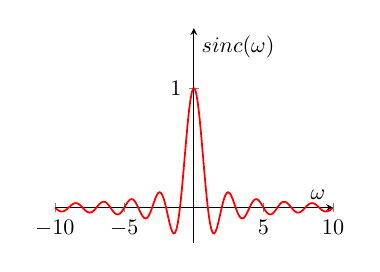
\begin{tikzpicture}[scale=0.8]
                        \begin{axis}[
                            domain=-10:10,
                            samples=200,
                            axis lines=middle,
                            xlabel={$\omega$},
                            ylabel={$sinc(\omega)$},
                            ymin=-0.3, ymax=1.5,
                            xmin=-10, xmax=10,
                            xtick={-10,-5,5,10},
                            ytick={1},
                            % grid=major,
                            height=5cm,
                            width=6cm
                        ]
                            \addplot[thick,red] {x == 0 ? 1 : sin(deg(pi*x))/(pi*x)};
                        \end{axis}
                    \end{tikzpicture}
                    \caption{$\mathcal{F} \{x_1(t)\}$ and $\mathcal{F} \{x_2(t)\}$}
                \end{subfigure}
            \end{figure}
        \end{block}
    }

    \only<4>{
        \begin{block}{Linearity}
            \begin{figure}[ht]
                \centering
                % 2 * rect(t) and Fourier Transform
                \begin{subfigure}[b]{0.45\textwidth}
                    \centering
                    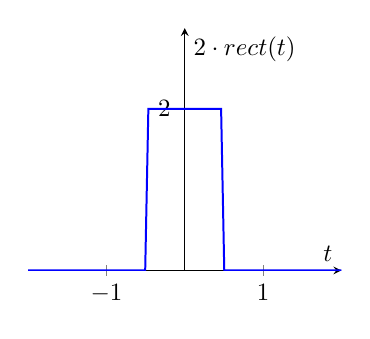
\begin{tikzpicture}[scale=0.9]
                        \begin{axis}[
                            domain=-2:2,
                            samples=100,
                            axis lines=middle,
                            xlabel={$t$},
                            ylabel={$2 \cdot rect(t)$},
                            ymin=0, ymax=3,
                            xmin=-2, xmax=2,
                            xtick={-1,0,1},
                            ytick={0,2},
                            height=5cm,
                            width=6cm
                        ]
                            \addplot[thick,blue] {2 * (abs(x) <= 0.5 ? 1 : 0)};
                        \end{axis}
                    \end{tikzpicture}
                    \caption{$2 \cdot x_1(t)$}
                \end{subfigure}
                \hfill
                % Fourier Transform of 2 * rect(t - 1)
                \begin{subfigure}[b]{0.45\textwidth}
                    \centering
                    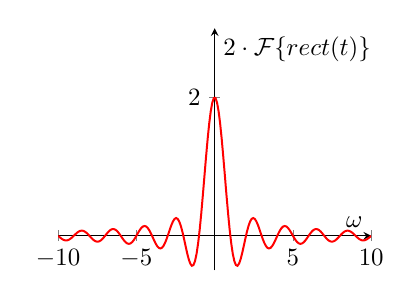
\begin{tikzpicture}[scale=0.9]
                        \begin{axis}[
                            domain=-10:10,
                            samples=200,
                            axis lines=middle,
                            xlabel={$\omega$},
                            ylabel={$2 \cdot \mathcal{F} \{rect(t)\}$},
                            ymin=-0.5, ymax=3,
                            xmin=-10, xmax=10,
                            xtick={-10,-5,5,10},
                            ytick={2},
                            height=5cm,
                            width=6cm
                        ]
                            \addplot[thick,red] {x == 0 ? 2 : 2 * sin(deg(pi*x))/(pi*x)};
                        \end{axis}
                    \end{tikzpicture}
                    \caption{$\mathcal{F} \{2 \cdot x_1(t)\}$}
                \end{subfigure}
            \end{figure}
            Here,
            \begin{equation*}
                \mathcal{F} \{\textcolor{blue}{2} \cdot x_1(t)\} = \textcolor{blue}{2} \cdot \mathcal{F} \{x_1(t)\}
            \end{equation*}
        \end{block}
    }

    \only<5>{
        \begin{block}{Linearity}
            \begin{figure}[ht]
                \centering
                % 3 * rect(t) and Fourier Transform
                \begin{subfigure}[b]{0.45\textwidth}
                    \centering
                    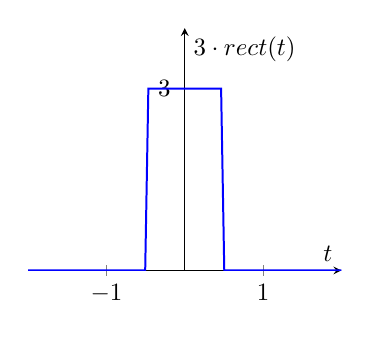
\begin{tikzpicture}[scale=0.9]
                        \begin{axis}[
                            domain=-2:2,
                            samples=100,
                            axis lines=middle,
                            xlabel={$t$},
                            ylabel={$3 \cdot rect(t)$},
                            ymin=0, ymax=4,
                            xmin=-2, xmax=2,
                            xtick={-1,0,1},
                            ytick={0,3},
                            height=5cm,
                            width=6cm
                        ]
                            \addplot[thick,blue] {3 * (abs(x) <= 0.5 ? 1 : 0)};
                        \end{axis}
                    \end{tikzpicture}
                    \caption{$3 \cdot x_2(t)$}
                \end{subfigure}
                \hfill
                % Fourier Transform of 2 * rect(t - 1)
                \begin{subfigure}[b]{0.45\textwidth}
                    \centering
                    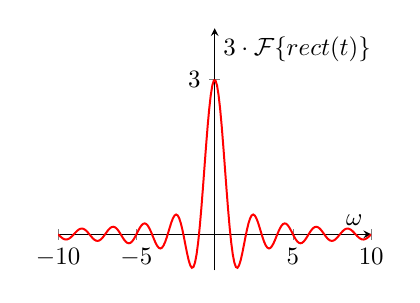
\begin{tikzpicture}[scale=0.9]
                        \begin{axis}[
                            domain=-10:10,
                            samples=200,
                            axis lines=middle,
                            xlabel={$\omega$},
                            ylabel={$3 \cdot \mathcal{F} \{rect(t)\}$},
                            ymin=-0.7, ymax=4,
                            xmin=-10, xmax=10,
                            xtick={-10,-5,5,10},
                            ytick={3},
                            height=5cm,
                            width=6cm
                        ]
                            \addplot[thick,red] {x == 0 ? 3 : 3 * sin(deg(pi*x))/(pi*x)};
                        \end{axis}
                    \end{tikzpicture}
                    \caption{$\mathcal{F} \{3 \cdot x_2(t)\}$}
                \end{subfigure}
            \end{figure}
            Here,
            \begin{equation*}
                \mathcal{F} \{\textcolor{red}{3} \cdot x_2(t)\} = \textcolor{red}{3} \cdot \mathcal{F} \{x_2(t)\}
            \end{equation*}
        \end{block}
    }

    \only<6>{
        \begin{block}{Linearity}
            \begin{figure}[ht]
                \centering
                \begin{subfigure}[b]{0.45\textwidth}
                    \centering
                    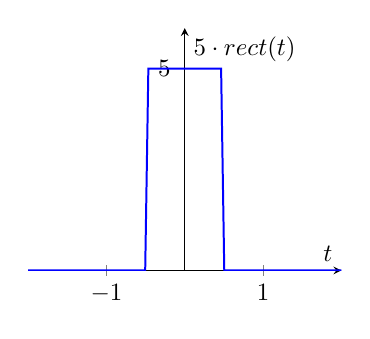
\begin{tikzpicture}[scale=0.9]
                        \begin{axis}[
                            domain=-2:2,
                            samples=100,
                            axis lines=middle,
                            xlabel={$t$},
                            ylabel={$5 \cdot rect(t)$},
                            ymin=0, ymax=6,
                            xmin=-2, xmax=2,
                            xtick={-1,0,1},
                            ytick={0,5},
                            height=5cm,
                            width=6cm
                        ]
                            \addplot[thick,blue] {5 * (abs(x) <= 0.5 ? 1 : 0)};
                        \end{axis}
                    \end{tikzpicture}
                    \caption{$2 \cdot x_1(t) + 3 \cdot x_2(t)$}
                \end{subfigure}
                \hfill
                % Fourier Transform of 2 * rect(t - 1)
                \begin{subfigure}[b]{0.45\textwidth}
                    \centering
                    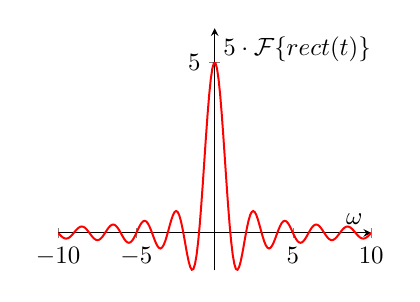
\begin{tikzpicture}[scale=0.9]
                        \begin{axis}[
                            domain=-10:10,
                            samples=200,
                            axis lines=middle,
                            xlabel={$\omega$},
                            ylabel={$5 \cdot \mathcal{F} \{rect(t)\}$},
                            ymin=-1.1, ymax=6,
                            xmin=-10, xmax=10,
                            xtick={-10,-5,5,10},
                            ytick={5},
                            height=5cm,
                            width=6cm
                        ]
                            \addplot[thick,red] {x == 0 ? 5 : 5 * sin(deg(pi*x))/(pi*x)};
                        \end{axis}
                    \end{tikzpicture}
                    \caption{$\mathcal{F} \{2 \cdot x_1(t)\} + \mathcal{F} \{3 \cdot x_2(t)\}$}
                \end{subfigure}
            \end{figure}
            Here,
            \begin{equation*}
                \mathcal{F} \{\textcolor{blue}{2} \cdot x_1(t) + \textcolor{red}{3} \cdot x_2(t)\} = \textcolor{blue}{2} \cdot \mathcal{F} \{x_1(t)\} + \textcolor{red}{3} \cdot \mathcal{F} \{x_2(t)\}
            \end{equation*}
        \end{block}
    }

    % Detailed content for Time Shifting
    \only<8>{
        \begin{block}{Time Shifting}
            If $x(t)$ is a signal with Fourier transform $X(\omega)$, then
            shifting the signal in time corresponds to a phase shift in its Fourier transform:
            \[
            x(t - \textcolor{red}{t_0}) \xrightarrow{\text{FT}} X(\omega)e^{-j\omega \textcolor{red}{t_0}}
            \]
        \end{block}
    }

    \only<9>{
        \begin{block}{Time Shifting}
            Let $x(t) = rect(t)$ be a signal with Fourier transform $X(\omega) = \mathcal{F} \{rect(t)\}$.
            
            \begin{figure}[ht]
                \centering
                % rect(t) and Fourier Transform (smaller images)
                \begin{subfigure}[b]{0.3\textwidth}
                    \centering
                    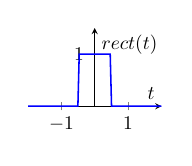
\begin{tikzpicture}[scale=0.7]
                        \begin{axis}[
                            domain=-2:2,
                            samples=100,
                            axis lines=middle,
                            xlabel={$t$},
                            ylabel={$rect(t)$},
                            ymin=0, ymax=1.5,
                            xmin=-2, xmax=2,
                            xtick={-1,0,1},
                            ytick={0,1},
                            height=3cm,
                            width=4cm
                        ]
                            \addplot[thick,blue] {abs(x) <= 0.5 ? 1 : 0};
                        \end{axis}
                    \end{tikzpicture}
                    \caption{$rect(t)$}
                \end{subfigure}
                \hspace{-0.5cm}
                \begin{subfigure}[b]{0.3\textwidth}
                    \centering
                    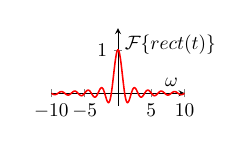
\begin{tikzpicture}[scale=0.7]
                        \begin{axis}[
                            domain=-10:10,
                            samples=200,
                            axis lines=middle,
                            xlabel={$\omega$},
                            ylabel={$\mathcal{F} \{rect(t)\}$},
                            ymin=-0.3, ymax=1.5,
                            xmin=-10, xmax=10,
                            xtick={-10,-5,5,10},
                            ytick={1},
                            height=3cm,
                            width=4cm
                        ]
                            \addplot[thick,red] {x == 0 ? 1 : sin(deg(pi*x))/(pi*x)};
                        \end{axis}
                    \end{tikzpicture}
                    \caption{$\mathcal{F} \{rect(t)\}$}
                \end{subfigure}
            \end{figure}
            \vspace{-0.5cm}
            \begin{figure}[ht]
                \centering
                % rect(t - 1) and Fourier Transform (normal size images)
                \begin{subfigure}[b]{0.45\textwidth}
                    \centering
                    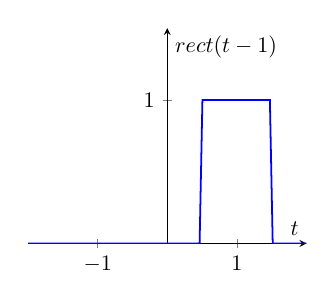
\begin{tikzpicture}[scale=0.8]
                        \begin{axis}[
                            domain=-2:2,
                            samples=100,
                            axis lines=middle,
                            xlabel={$t$},
                            ylabel={$rect(t - 1)$},
                            ymin=0, ymax=1.5,
                            xmin=-2, xmax=2,
                            xtick={-1,0,1},
                            ytick={0,1},
                            height=5cm,
                            width=6cm
                        ]
                            \addplot[thick,blue] {abs(x - 1) <= 0.5 ? 1 : 0};
                        \end{axis}
                    \end{tikzpicture}
                    \caption{$rect(t - 1)$}
                \end{subfigure}
                \hfill
                \begin{subfigure}[b]{0.45\textwidth}
                    \centering
                    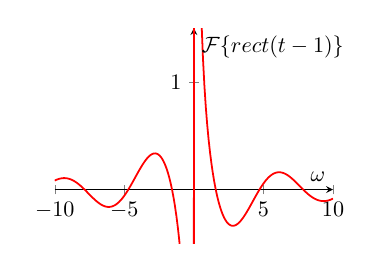
\begin{tikzpicture}[scale=0.8]
                        \begin{axis}[
                            domain=-10:10,
                            samples=200,
                            axis lines=middle,
                            xlabel={$\omega$},
                            ylabel={$\mathcal{F} \{rect(t - 1)\}$},
                            ymin=-0.5, ymax=1.5,
                            xmin=-10, xmax=10,
                            xtick={-10,-5,5,10},
                            ytick={1},
                            height=5cm,
                            width=6cm
                        ]
                            \addplot[thick,red] {cos(deg(x))/x};
                        \end{axis}
                    \end{tikzpicture}
                    \caption{$\mathcal{F} \{rect(t - 1)\}$}
                \end{subfigure}
            \end{figure}
        \end{block}
    }


    \only<10>{
        \begin{block}{Time Shifting}
            Here,
            \begin{equation*}
                rect(t - \textcolor{red}{1}) \xrightarrow{\text{FT}} X(\omega)e^{-j\omega \textcolor{red}{1}}
            \end{equation*}
        \end{block}
    }

    % Detailed content for Time Scaling
    \only<12>{
        \begin{block}{Time Scaling}
            If $x(t)$ is a signal with Fourier transform $X(\omega)$, then
            stretching or compressing a signal in time inversely scales its frequency spectrum:
            \[
            x(\textcolor{red}{a} t) \xrightarrow{\text{FT}} \frac{1}{|\textcolor{red}{a}|}X\left(\frac{\omega}{\textcolor{red}{a}}\right)
            \]
        \end{block}
    }

    \only<13>{
        \begin{block}{Time Scaling}
            Let $x(t) = rect(t)$ be a signal with Fourier transform $X(\omega) = \mathcal{F} \{rect(t)\}$.
            \begin{figure}
                \centering
                % Rect function
                \begin{subfigure}[b]{0.3\textwidth}
                    \centering
                    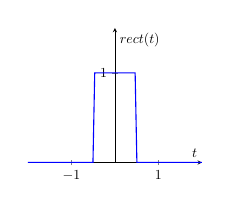
\begin{tikzpicture}[scale=0.5]
                        \begin{axis}[
                            domain=-2:2,
                            samples=100,
                            axis lines=middle,
                            xlabel={$t$},
                            ylabel={$rect(t)$},
                            ymin=0, ymax=1.5,
                            xmin=-2, xmax=2,
                            xtick={-1,0,1},
                            ytick={0,1},
                            % grid=major,
                            height=5cm,
                            width=6cm
                        ]
                            \addplot[thick,blue] {abs(x) <= 0.5 ? 1 : 0};
                        \end{axis}
                    \end{tikzpicture}
                    \caption{$x(t)$}
                \end{subfigure}
                \hspace{-0.5cm}
                % Sinc function
                \begin{subfigure}[b]{0.3\textwidth}
                    \centering
                    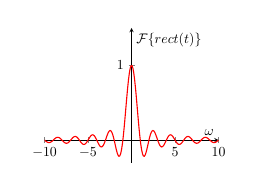
\begin{tikzpicture}[scale=0.5]
                        \begin{axis}[
                            domain=-10:10,
                            samples=200,
                            axis lines=middle,
                            xlabel={$\omega$},
                            ylabel={$\mathcal{F} \{rect(t)\}$},
                            ymin=-0.3, ymax=1.5,
                            xmin=-10, xmax=10,
                            xtick={-10,-5,5,10},
                            ytick={1},
                            % grid=major,
                            height=5cm,
                            width=6cm
                        ]
                            \addplot[thick,red] {x == 0 ? 1 : sin(deg(pi*x))/(pi*x)};
                        \end{axis}
                    \end{tikzpicture}
                    \caption{$\mathcal{F} \{x(t)\}$}
                \end{subfigure}
            \end{figure}
            \vspace{-0.5cm}
            \begin{figure}
                \centering
                % Time domain signal rect(2t)
                \begin{subfigure}[b]{0.45\textwidth}
                    \centering
                    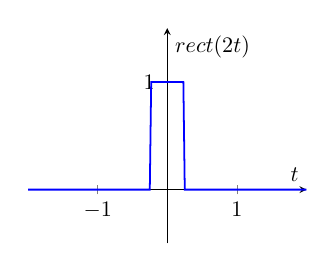
\begin{tikzpicture}[scale=0.8]
                        \begin{axis}[
                            domain=-2:2,
                            samples=200,
                            axis lines=middle,
                            xlabel={$t$},
                            ylabel={$rect(2t)$},
                            ymin=-0.5, ymax=1.5,
                            xmin=-2, xmax=2,
                            xtick={-1,0,1},
                            ytick={0,1},
                            height=5cm,
                            width=6cm
                        ]
                            \addplot[thick,blue] {abs(2*x) <= 0.5 ? 1 : 0};
                        \end{axis}
                    \end{tikzpicture}
                    \caption{$x(2t)$}
                \end{subfigure}
                \hfill
                % Fourier Transform of rect(2t)
                \begin{subfigure}[b]{0.45\textwidth}
                    \centering
                    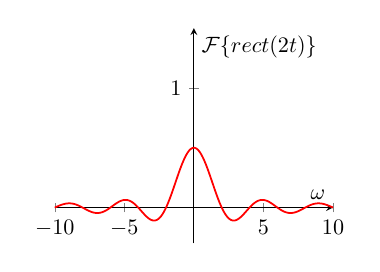
\begin{tikzpicture}[scale=0.8]
                        \begin{axis}[
                            domain=-10:10,
                            samples=200,
                            axis lines=middle,
                            xlabel={$\omega$},
                            ylabel={$\mathcal{F} \{rect(2t)\}$},
                            ymin=-0.3, ymax=1.5,
                            xmin=-10, xmax=10,
                            xtick={-10,-5,0,5,10},
                            ytick={1},
                            height=5cm,
                            width=6cm
                        ]
                            \addplot[thick,red] {(sin(deg(pi*x/2))/(pi*x/2))/2};
                        \end{axis}
                    \end{tikzpicture}
                    \caption{$\mathcal{F} \{x(2t)\}$}
                \end{subfigure}
            \end{figure}
        \end{block}
    }

    \only<14>{
        \begin{block}{Time Scaling}
            Here,
            \begin{equation*}
                rect(2t) \xrightarrow{\text{FT}} \frac{1}{2}sinc(\frac{\omega}{2})
            \end{equation*}
        \end{block}
    }

    % Detailed content for Time Reversal
    \only<16>{
        \begin{block}{Time Reversal}
            If $x(t)$ is a signal with Fourier transform $X(\omega)$, then
            \textcolor{blue}{time reversal} of the signal in the time domain corresponds to \textcolor{blue}{frequency reversal} in the frequency domain:
            \[
            x(\textcolor{red}{-} t) \xrightarrow{\text{FT}} X(\textcolor{red}{-} \omega)
            \]
        \end{block}
    }

    \only<17>{
        \begin{block}{Time Reversal}
            Let $x(t) = rect(t)$ be a signal with Fourier transform $X(\omega) = \mathcal{F} \{rect(t)\}$.
            \begin{figure}
                \centering
                % Rect function
                \begin{subfigure}[b]{0.3\textwidth}
                    \centering
                    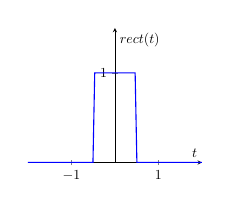
\begin{tikzpicture}[scale=0.5]
                        \begin{axis}[
                            domain=-2:2,
                            samples=100,
                            axis lines=middle,
                            xlabel={$t$},
                            ylabel={$rect(t)$},
                            ymin=0, ymax=1.5,
                            xmin=-2, xmax=2,
                            xtick={-1,0,1},
                            ytick={0,1},
                            % grid=major,
                            height=5cm,
                            width=6cm
                        ]
                            \addplot[thick,blue] {abs(x) <= 0.5 ? 1 : 0};
                        \end{axis}
                    \end{tikzpicture}
                    \caption{$x(t)$}
                \end{subfigure}
                \hspace{-0.5cm}
                % Sinc function
                \begin{subfigure}[b]{0.3\textwidth}
                    \centering
                    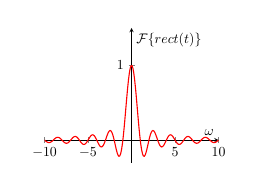
\begin{tikzpicture}[scale=0.5]
                        \begin{axis}[
                            domain=-10:10,
                            samples=200,
                            axis lines=middle,
                            xlabel={$\omega$},
                            ylabel={$\mathcal{F} \{rect(t)\}$},
                            ymin=-0.3, ymax=1.5,
                            xmin=-10, xmax=10,
                            xtick={-10,-5,5,10},
                            ytick={1},
                            % grid=major,
                            height=5cm,
                            width=6cm
                        ]
                            \addplot[thick,red] {x == 0 ? 1 : sin(deg(pi*x))/(pi*x)};
                        \end{axis}
                    \end{tikzpicture}
                    \caption{$\mathcal{F} \{x(t)\}$}
                \end{subfigure}
            \end{figure}
            \vspace{-0.5cm}
            \begin{figure}[ht]
                \centering
                % Time domain signal rect(-t)
                \begin{subfigure}[b]{0.45\textwidth}
                    \centering
                    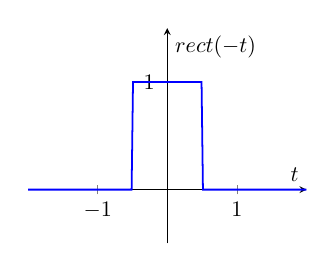
\begin{tikzpicture}[scale=0.8]
                        \begin{axis}[
                            domain=-2:2,
                            samples=200,
                            axis lines=middle,
                            xlabel={$t$},
                            ylabel={$rect(-t)$},
                            ymin=-0.5, ymax=1.5,
                            xmin=-2, xmax=2,
                            xtick={-1,0,1},
                            ytick={0,1},
                            height=5cm,
                            width=6cm
                        ]
                            \addplot[thick,blue] {abs(-x) <= 0.5 ? 1 : 0};
                        \end{axis}
                    \end{tikzpicture}
                    \caption{$x(-t)$}
                \end{subfigure}
                \hfill
                % Fourier Transform of rect(-t)
                \begin{subfigure}[b]{0.45\textwidth}
                    \centering
                    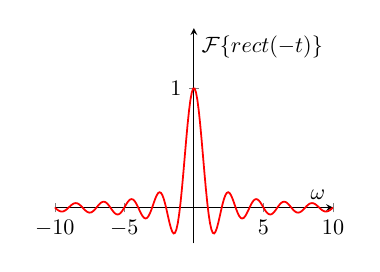
\begin{tikzpicture}[scale=0.8]
                        \begin{axis}[
                            domain=-10:10,
                            samples=200,
                            axis lines=middle,
                            xlabel={$\omega$},
                            ylabel={$\mathcal{F} \{rect(-t)\}$},
                            ymin=-0.3, ymax=1.5,
                            xmin=-10, xmax=10,
                            xtick={-10,-5,0,5,10},
                            ytick={1},
                            height=5cm,
                            width=6cm
                        ]
                            \addplot[thick,red] {(sin(deg(pi*x))/(pi*x))};
                        \end{axis}
                    \end{tikzpicture}
                    \caption{$\mathcal{F} \{x(-t)\}$}
                \end{subfigure}
            \end{figure}
        \end{block}
    }

    \only<18>{
        \begin{block}{Time Reversal}
            Both functions are even hence they remain same.
            Here,
            \begin{equation*}
                rect(-t) \xrightarrow{\text{FT}} \mathcal{F}\{x(-t)\}
            \end{equation*}
        \end{block}
    }

    % Detailed content for Time Differentiation
    \only<20>{
        \begin{block}{Differentiation}
            If $x(t)$ is a signal with Fourier transform $X(\omega)$, then
            differentiation in the time domain corresponds to multiplication by $j\omega$ in the frequency domain:
            \[
            \frac{d}{dt}x(t) \xrightarrow{\text{FT}} \textcolor{red}{j\omega} X(\omega)
            \]
        \end{block}
    }

    \only<21>{
        \begin{block}{Differentiation}
            Let $x(t) = rect(t)$ be a signal with Fourier transform $X(\omega) = \mathcal{F} \{rect(t)\}$.
            \begin{figure}
                \centering
                % Rect function
                \begin{subfigure}[b]{0.3\textwidth}
                    \centering
                    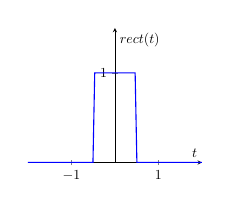
\begin{tikzpicture}[scale=0.5]
                        \begin{axis}[
                            domain=-2:2,
                            samples=100,
                            axis lines=middle,
                            xlabel={$t$},
                            ylabel={$rect(t)$},
                            ymin=0, ymax=1.5,
                            xmin=-2, xmax=2,
                            xtick={-1,0,1},
                            ytick={0,1},
                            % grid=major,
                            height=5cm,
                            width=6cm
                        ]
                            \addplot[thick,blue] {abs(x) <= 0.5 ? 1 : 0};
                        \end{axis}
                    \end{tikzpicture}
                    \caption{$x(t)$}
                \end{subfigure}
                \hspace{-0.5cm}
                % Sinc function
                \begin{subfigure}[b]{0.3\textwidth}
                    \centering
                    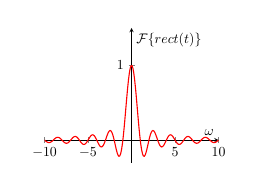
\begin{tikzpicture}[scale=0.5]
                        \begin{axis}[
                            domain=-10:10,
                            samples=200,
                            axis lines=middle,
                            xlabel={$\omega$},
                            ylabel={$\mathcal{F} \{rect(t)\}$},
                            ymin=-0.3, ymax=1.5,
                            xmin=-10, xmax=10,
                            xtick={-10,-5,5,10},
                            ytick={1},
                            % grid=major,
                            height=5cm,
                            width=6cm
                        ]
                            \addplot[thick,red] {x == 0 ? 1 : sin(deg(pi*x))/(pi*x)};
                        \end{axis}
                    \end{tikzpicture}
                    \caption{$\mathcal{F} \{x(t)\}$}
                \end{subfigure}
            \end{figure}
            \vspace{-0.5cm}
            \begin{figure}
                \centering
                % Differentiated signal
                \begin{subfigure}[b]{0.45\textwidth}
                    \centering
                    \begin{tikzpicture}[scale=0.8]
                        \begin{axis}[
                            domain=-2:2,
                            samples=200,
                            axis lines=middle,
                            xlabel={$t$},
                            ylabel={$\frac{d}{dt}rect(t)$},
                            ymin=-1.5, ymax=1.5,
                            xmin=-2, xmax=2,
                            xtick={-1,0,1},
                            ytick={-1,0,1},
                            height=5cm,
                            width=6cm
                        ]
                            \addplot[only marks,mark=triangle*,mark options={scale=2,fill=blue}] coordinates {(0.5,-1)};
                            \addplot[only marks,mark=triangle*,mark options={scale=2,fill=red}] coordinates {(-0.5,1)};
                        \end{axis}
                    \end{tikzpicture}
                    \caption{$\frac{d}{dt}x(t)$}
                \end{subfigure}
                \hfill
                % Fourier Transform of differentiated signal
                \begin{subfigure}[b]{0.45\textwidth}
                    \centering
                    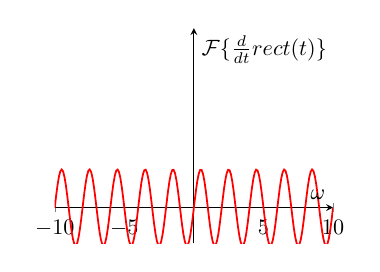
\begin{tikzpicture}[scale=0.8]
                        \begin{axis}[
                            domain=-10:10,
                            samples=200,
                            axis lines=middle,
                            xlabel={$\omega$},
                            ylabel={$\mathcal{F} \{\frac{d}{dt}rect(t)\}$},
                            ymin=-0.3, ymax=1.5,
                            xmin=-10, xmax=10,
                            xtick={-10,-5,0,5,10},
                            ytick={0},
                            height=5cm,
                            width=6cm
                        ]
                            \addplot[thick,red] {x*sin(deg(pi*x))/(pi*x)};
                        \end{axis}
                    \end{tikzpicture}
                    \caption{$\mathcal{F} \{\frac{d}{dt}x(t)\}$}
                \end{subfigure}
            \end{figure}
        \end{block}
    }

    % Detailed content for Time Integration
    \only<23>{
        \begin{block}{Integration}
            If $x(t)$ is a signal with fourier transform $X(\omega)$, then
            integration in the time domain corresponds to multiplication by $\frac{1}{j\omega}$ in the frequency domain:
            \[
            \int x(t)dt \xrightarrow{\text{FT}} \textcolor{red}{\frac{1}{j\omega}} X(\omega)
            \]
        \end{block}
    }

    \only<24>{
        \begin{block}{Integration}
            Let $x(t) = rect(t)$ be a signal with Fourier transform $X(\omega) = \mathcal{F} \{rect(t)\}$.
            \begin{figure}
                \centering
                % Rect function
                \begin{subfigure}[b]{0.3\textwidth}
                    \centering
                    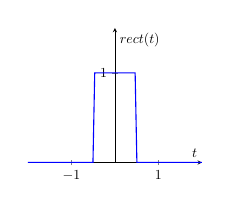
\begin{tikzpicture}[scale=0.5]
                        \begin{axis}[
                            domain=-2:2,
                            samples=100,
                            axis lines=middle,
                            xlabel={$t$},
                            ylabel={$rect(t)$},
                            ymin=0, ymax=1.5,
                            xmin=-2, xmax=2,
                            xtick={-1,0,1},
                            ytick={0,1},
                            % grid=major,
                            height=5cm,
                            width=6cm
                        ]
                            \addplot[thick,blue] {abs(x) <= 0.5 ? 1 : 0};
                        \end{axis}
                    \end{tikzpicture}
                    \caption{Signal}
                \end{subfigure}
                \hfill
                % Sinc function
                \begin{subfigure}[b]{0.3\textwidth}
                    \centering
                    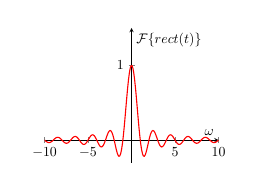
\begin{tikzpicture}[scale=0.5]
                        \begin{axis}[
                            domain=-10:10,
                            samples=200,
                            axis lines=middle,
                            xlabel={$\omega$},
                            ylabel={$\mathcal{F} \{rect(t)\}$},
                            ymin=-0.3, ymax=1.5,
                            xmin=-10, xmax=10,
                            xtick={-10,-5,5,10},
                            ytick={1},
                            % grid=major,
                            height=5cm,
                            width=6cm
                        ]
                            \addplot[thick,red] {x == 0 ? 1 : sin(deg(pi*x))/(pi*x)};
                        \end{axis}
                    \end{tikzpicture}
                    \caption{$\mathcal{F} \{rect(t)\}$}
                \end{subfigure}
            \end{figure}
            \vspace{-0.5cm}
            \begin{figure}
                \centering
                % Integrated signal
                \begin{subfigure}[b]{0.45\textwidth}
                    \centering
                    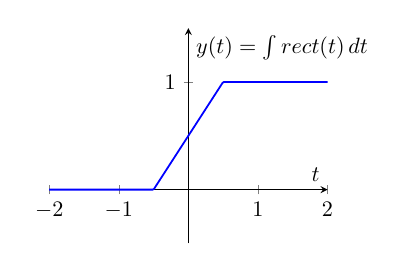
\begin{tikzpicture}[scale=0.8]
                        \begin{axis}[
                            domain=-2:2,
                            samples=200,
                            axis lines=middle,
                            xlabel={$t$},
                            ylabel={$y(t) = \int rect(t) \, dt$},
                            ymin=-0.5, ymax=1.5,
                            xmin=-2, xmax=2,
                            xtick={-2,-1,0,1,2},
                            ytick={0,1},
                            height=5cm,
                            width=6cm
                        ]
                            \addplot[thick,blue] {x <= -0.5 ? 0 : (x < 0.5 ? x + 0.5 : 1)};
                        \end{axis}
                    \end{tikzpicture}
                    \caption{$y(t) = \int x(t) dt$}
                \end{subfigure}
                \hfill
                % Fourier Transform of integrated signal
                \begin{subfigure}[b]{0.45\textwidth}
                    \centering
                    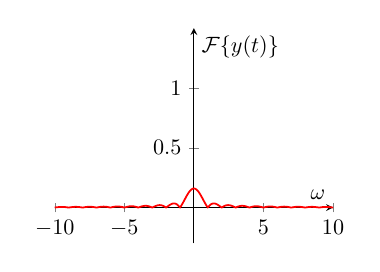
\begin{tikzpicture}[scale=0.8]
                        \begin{axis}[
                            domain=-10:10,
                            samples=200,
                            axis lines=middle,
                            xlabel={$\omega$},
                            ylabel={$\mathcal{F} \{y(t)\}$},
                            ymin=-0.3, ymax=1.5,
                            xmin=-10, xmax=10,
                            xtick={-10,-5,0,5,10},
                            ytick={0,0.5,1},
                            height=5cm,
                            width=6cm
                        ]
                            \addplot[
                                domain=-10:10,
                                samples=1000,
                                thick,
                                red
                            ] {abs(sin(deg(pi*x))/(pi*x)/(2*pi))} node[pos=0.75, above] {};
                        \end{axis}
                    \end{tikzpicture}
                    \caption{$\mathcal{F} \{y(t)\}$}
                \end{subfigure}
            \end{figure}
        \end{block}
    }

    % Detailed content for Time Convolution
    \only<26>{
        \begin{block}{Convolution}
            If $x(t)$ and $y(t)$ are two signals with fourier transform $X(\omega)$ and $Y(\omega)$, then
            convolution of the two signals in the time domain corresponds to multiplication in the frequency domain:
            \[
            x(t) \textcolor{red}{*} y(t) \xrightarrow{\text{FT}} X(\omega)\textcolor{red}{\cdot} Y(\omega)
            \]
        \end{block}
    }

    \only<27>{
        \begin{block}{Convolution}
            Let $x(t) = rect(t)$ and $y(t) = rect(t)$ be signals with Fourier transforms $X(\omega) = \mathcal{F} \{rect(t)\}$ and $Y(\omega) = \mathcal{F} \{rect(t)\}$. The convolution in the time domain corresponds to the product in the frequency domain:
            \[
            z(t) = x(t) * y(t) \quad \leftrightarrow \quad Z(\omega) = X(\omega) \cdot Y(\omega).
            \]
            \begin{figure}
                \centering
                % Rect function
                \begin{subfigure}[b]{0.45\textwidth}
                    \centering
                    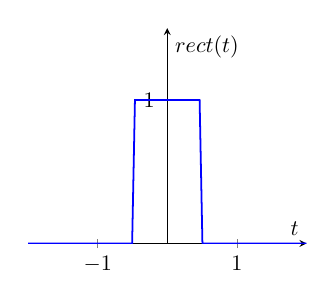
\begin{tikzpicture}[scale=0.8]
                        \begin{axis}[
                            domain=-2:2,
                            samples=100,
                            axis lines=middle,
                            xlabel={$t$},
                            ylabel={$rect(t)$},
                            ymin=0, ymax=1.5,
                            xmin=-2, xmax=2,
                            xtick={-1,0,1},
                            ytick={0,1},
                            height=5cm,
                            width=6cm
                        ]
                            \addplot[thick,blue] {abs(x) <= 0.5 ? 1 : 0};
                        \end{axis}
                    \end{tikzpicture}
                    \caption{$rect(t)$}
                \end{subfigure}
                \hfill
                % Sinc function
                \begin{subfigure}[b]{0.45\textwidth}
                    \centering
                    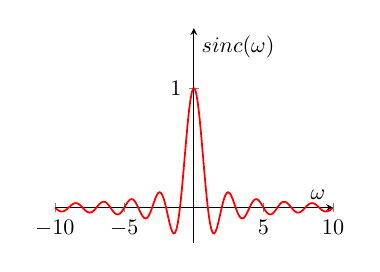
\begin{tikzpicture}[scale=0.8]
                        \begin{axis}[
                            domain=-10:10,
                            samples=200,
                            axis lines=middle,
                            xlabel={$\omega$},
                            ylabel={$sinc(\omega)$},
                            ymin=-0.3, ymax=1.5,
                            xmin=-10, xmax=10,
                            xtick={-10,-5,5,10},
                            ytick={1},
                            height=5cm,
                            width=6cm
                        ]
                            \addplot[thick,red] {x == 0 ? 1 : sin(deg(pi*x))/(pi*x)};
                        \end{axis}
                    \end{tikzpicture}
                    \caption{$\mathcal{F} \{rect(t)\}$}
                \end{subfigure}
            \end{figure}
        \end{block}
    }

    \only<28>{
        \begin{block}{Convolution}
            \begin{figure}
                \centering
                % Convolution of two rect functions
                \begin{subfigure}[b]{0.45\textwidth}
                    \centering
                    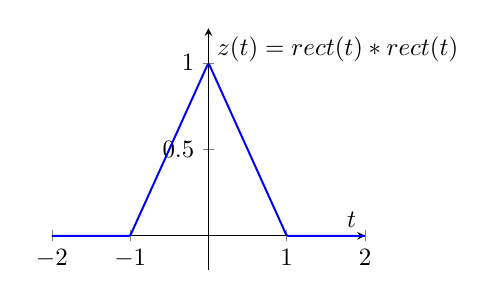
\begin{tikzpicture}[scale=0.9]
                        \begin{axis}[
                            domain=-2:2,
                            samples=200,
                            axis lines=middle,
                            xlabel={$t$},
                            ylabel={$z(t) = rect(t) * rect(t)$},
                            ymin=-0.2, ymax=1.2,
                            xmin=-2, xmax=2,
                            xtick={-2,-1,0,1,2},
                            ytick={0,0.5,1},
                            height=5cm,
                            width=6cm
                        ]
                            \addplot[thick,blue] {abs(x) <= 1 ? (1 - abs(x)) : 0};
                        \end{axis}
                    \end{tikzpicture}
                    \caption{$z(t) = rect(t) * rect(t)$}
                \end{subfigure}
                \hfill
                % Fourier Transform of convolution of two rect functions
                \begin{subfigure}[b]{0.45\textwidth}
                    \centering
                    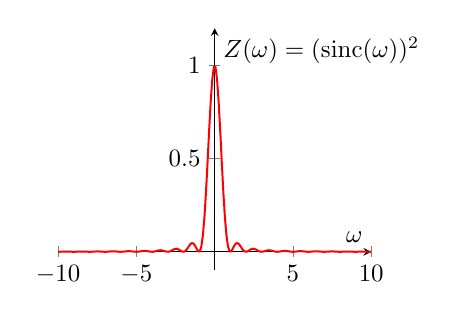
\begin{tikzpicture}[scale=0.9]
                        \begin{axis}[
                            domain=-10:10,
                            samples=200,
                            axis lines=middle,
                            xlabel={$\omega$},
                            ylabel={$Z(\omega) = (\text{sinc}(\omega))^2$},
                            ymin=-0.1, ymax=1.2,
                            xmin=-10, xmax=10,
                            xtick={-10,-5,0,5,10},
                            ytick={0,0.5,1},
                            height=5cm,
                            width=6cm
                        ]
                            \addplot[thick,red] {x == 0 ? 1 : (sin(deg(pi*x))/(pi*x))^2};
                        \end{axis}
                    \end{tikzpicture}
                    \caption{$Z(\omega) = \mathcal{F} \{z(t)\}$}
                \end{subfigure}
            \end{figure}
            Here,
            \begin{equation*}
                rect(t) \textcolor{red}{*} rect(t) = X(\omega)\textcolor{red}{\cdot} Y(\omega)
            \end{equation*}
        \end{block}
    }
\end{frame}

\begin{frame}{Fourier Transform Properties (Table 1)}
    \begin{table}[ht]
    \centering
    \renewcommand{\arraystretch}{1.5}  % Adjust row height
    \small  % Reduce font size
        \begin{tabular}{|>{\columncolor{rowcolor1}}p{3cm}|>{\columncolor{rowcolor1}}p{3.5cm}|>{\columncolor{rowcolor1}}p{4.5cm}|}
            \hline
            \textbf{Property} & \textbf{Time Domain} & \textbf{Fourier Transform} \\
            \hline
            \rowcolor{rowcolor2}
            Linearity & \( x(t) = A x_1(t) + B x_2(t) \) & \( X(j\omega) = A X_1(j\omega) + B X_2(j\omega) \) \\
            \hline
            Time Shifting & \( x(t - t_0) \) & \( e^{-j\omega t_0} X(j\omega) \) \\
            \hline
            \rowcolor{rowcolor2}
            Conjugation & \( x^*(t) \) & \( X^*(-j\omega) \) \\
            \hline
            Differentiation in Time & \( \frac{d^n x(t)}{dt^n} \) & \( (j\omega)^n X(j\omega) \) \\
            \hline
            \rowcolor{rowcolor2}
            Differentiation in Frequency & \( -jt x(t) \) & \( \frac{dX(j\omega)}{d\omega} \) \\
            \hline
            Time Integration & \( \int_{-\infty}^t x(\tau)d\tau \) & \( \frac{1}{j\omega} X(j\omega) + \pi X(0)\delta(\omega) \) \\
            \hline
        \end{tabular}
    \end{table}
\end{frame}

\begin{frame}{Fourier Transform Properties (Table 2)}
    \begin{table}[ht]
    \centering
    \renewcommand{\arraystretch}{1.5}  % Adjust row height
    \small  % Reduce font size
        \begin{tabular}{|>{\columncolor{rowcolor1}}c|>{\columncolor{rowcolor1}}c|>{\columncolor{rowcolor1}}c|}
            \hline
            \textbf{Property} & \textbf{Time Domain} & \textbf{Fourier Transform} \\
            \hline
            \rowcolor{rowcolor2}
            Time Scaling & \( x(at) \) & \( \frac{1}{|a|} X\left(\frac{j\omega}{a}\right) \) \\
            \hline
            Time Reversal & \( x(-t) \) & \( X(-j\omega) \) \\
            \hline
            \rowcolor{rowcolor2}
            Frequency Shifting & \( x(t) e^{j\omega_0 t} \) & \( X(j(\omega - \omega_0)) \) \\
            \hline
            Duality & \( X(t) \) & \( 2\pi x(-j\omega) \) \\
            \hline
            \rowcolor{rowcolor2}
            Time Convolution & \( x(t) * h(t) \) & \( X(j\omega) H(j\omega) \) \\
            \hline
            Parseval's Theorem & \( \int_{-\infty}^\infty |x(t)|^2 dt \) & \( \frac{1}{2\pi} \int_{-\infty}^\infty |X(j\omega)|^2 d\omega \) \\
            \hline
            \rowcolor{rowcolor2}
            Modulation & \( z(t) = x(t) y(t) \) & \( Z(\omega) = \frac{1}{2\pi} X(j\omega) * Y(j\omega) \) \\
            \hline
        \end{tabular}
    \end{table}
\end{frame}

\begin{frame}{Fourier Transform Table}
    \begin{table}[ht]
    \centering
    \renewcommand{\arraystretch}{1.5}  % Adjust row height
        \begin{tabular}{|>{\columncolor{rowcolor1}}c|>{\columncolor{rowcolor1}}c|}
            \hline
            \textbf{Signal in Time Domain} & \textbf{Fourier Transform} \\
            \hline
            \rowcolor{rowcolor2}
            \( \delta(t) \) & \( 1 \) \\
            \hline
            \( u(t) \) & \( \frac{1}{j\omega} + \pi \delta(\omega) \) \\
            \hline
            \rowcolor{rowcolor2}
            \( \delta(t - t_0) \) & \( e^{-j\omega t_0} \) \\
            \hline
            \( t e^{-a t} u(t) \) & \( \frac{1}{(a + j\omega)^2} \) \\
            \hline
            \rowcolor{rowcolor2}
            \( u(-t) \) & \( \pi \delta(\omega) - \frac{1}{j\omega} \) \\
            \hline
            \( e^{at} u(-t) \) & \( \frac{1}{a - j\omega} \) \\
            \hline
        \end{tabular}
    \end{table}
\end{frame}

\begin{frame}{Fourier Transform Table}
    \begin{table}[ht]
    \centering
    \renewcommand{\arraystretch}{1.5}  % Adjust row height
        \begin{tabular}{|>{\columncolor{rowcolor1}}c|>{\columncolor{rowcolor1}}c|}
            \hline
            \textbf{Signal in Time Domain} & \textbf{Fourier Transform} \\
            \hline
            \rowcolor{rowcolor2}
            \( e^{-a|t|} \) & \( \frac{2a}{a^2 + \omega^2} \) \\
            \hline
            \( \cos(\omega_0 t) \) & \( \pi [\delta(\omega - \omega_0) + \delta(\omega + \omega_0)] \) \\
            \hline
            \rowcolor{rowcolor2}
            \( \sin(\omega_0 t) \) & \( -j \pi [\delta(\omega - \omega_0) - \delta(\omega + \omega_0)] \) \\
            \hline
            \( \frac{1}{a^2 + t^2} \) & \( e^{-a|\omega|} \) \\
            \hline
            \rowcolor{rowcolor2}
            \( \text{Sgn}(t) \) & \( \frac{2}{j\omega} \) \\
            \hline
            \( 1 \, \text{(for all t)} \) & \( 2\pi \delta(\omega) \) \\
            \hline
        \end{tabular}
    \end{table}
    \footnote{https://www.philadelphia.edu.jo/academics/qhamarsheh/uploads/Lecture}
\end{frame}

\begin{frame}
    \textcolor{green}{\textbf{Application of Fourier transform}}
\end{frame}

\begin{frame}
    \frametitle{Application of Fourier Transform include}
    \begin{itemize}[label=$\star$, itemsep=7pt, parsep=0pt, topsep=10pt]
      \item<1-> Signal Processing
      \item<2-> Image Processing
      \item<3-> Filtering: 
          \begin{itemize}
              \item<4-> High Pass Filter 
              \item<5-> Low Pass Filter 
              \item<6-> Band Pass Filter
              \item <7-> Band Reject Filter
          \end{itemize}
      \item<8-> Audio Processing
      \item<9-> Reducing Noise
      \item<10-> Telecommunications
      \item<12-> Representing wave propagation
    \end{itemize}
  \end{frame}
  
  \begin{frame}
    \frametitle{Application of Fourier Transform: \textcolor{yellow}{Signal Processing}}
    \begin{itemize} [label=$\star$, itemsep=4pt, parsep=0pt, topsep=10pt]
        \item<1-> \textbf{\textcolor{red}{Signal Decomposing into Frequencies Components}}
    \end{itemize}
     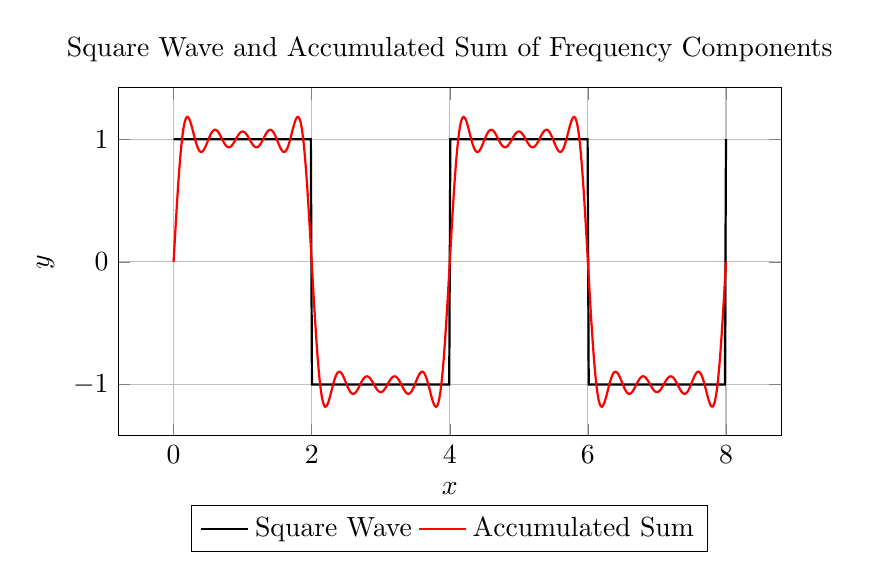
\begin{tikzpicture}
          \begin{axis}[
              title={Square Wave and Accumulated Sum of Frequency Components},
              xlabel={$x$},
              ylabel={$y$},
              grid=both,
              legend style={at={(0.5,-0.2)}, anchor=north, legend columns=-1},
              width=10cm,
              height=6cm
          ]
              % Square wave (Ideal target)
              \addplot[domain=0:8, samples=500, thick, black] 
               {mod(abs(x), 4) < 2 ? 1 : -1};
              % \addlegendentry{Square Wave}
  
              % Accumulated Fourier components
              \addplot[domain=0:8, samples=500, thick, red] 
                 {4/pi * (sin(deg(pi*x/2)) + 1/3*sin(deg(3*pi*x/2)) + 1/5*sin(deg(5*pi*x/2)) + 1/7*sin(deg(7*pi*x/2)) + 1/9*sin(deg(9*pi*x/2)))};
              % \addlegendentry{Accumulated Sum (5 terms)}
              \addlegendentry{Square Wave}
              \addlegendentry{Accumulated Sum}
          \end{axis}
      \end{tikzpicture}
  \end{frame}
  
  \begin{frame}
    \frametitle{Application of Fourier Transform: \textcolor{yellow}{Signal Processing}}
    \begin{itemize} [label=$\star$, itemsep=4pt, parsep=0pt, topsep=10pt]
        \item<1-> \textbf{\textcolor{red}{Signal Decomposing into Frequencies Components}}
    \end{itemize}
    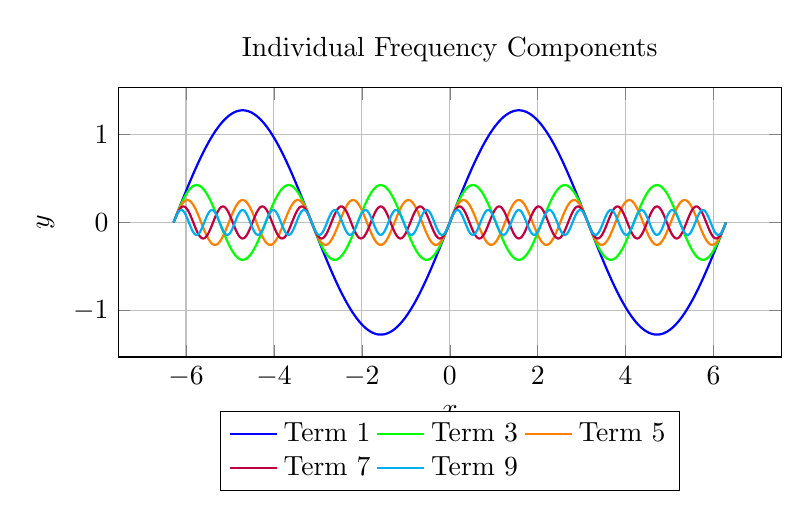
\begin{tikzpicture}
          \begin{axis}[
              title={Individual Frequency Components},
              xlabel={$x$},
              ylabel={$y$},
              grid=both,
              width=10cm,
              height=5cm,
              legend style={at={(0.5,-0.2)}, anchor=north, legend columns=3}
          ]
              % Individual sinusoidal components
              \addplot[domain=-2*pi:2*pi, samples=500, thick, blue] 
                  {4/pi * sin(deg(x))};
              \addlegendentry{Term 1}
  
              \addplot[domain=-2*pi:2*pi, samples=500, thick, green] 
                  {4/(3*pi) * sin(deg(3*x))};
              \addlegendentry{Term 3}
  
              \addplot[domain=-2*pi:2*pi, samples=500, thick, orange] 
                  {4/(5*pi) * sin(deg(5*x))};
              \addlegendentry{Term 5}
  
              \addplot[domain=-2*pi:2*pi, samples=500, thick, purple] 
                  {4/(7*pi) * sin(deg(7*x))};
              \addlegendentry{Term 7}
  
              \addplot[domain=-2*pi:2*pi, samples=500, thick, cyan] 
                  {4/(9*pi) * sin(deg(9*x))};
              \addlegendentry{Term 9}
          \end{axis}
      \end{tikzpicture}
  \end{frame}
  
  \begin{frame}
     \frametitle{Application of Fourier Transform: \textcolor{yellow}{Signal Processing}}
    \begin{itemize} [label=$\star$, itemsep=4pt, parsep=0pt, topsep=10pt]
        \item<1-> \textbf{\textcolor{red}{Signal Decomposing into Frequencies Components}}
    \end{itemize}
    \begin{figure}
        \centering
        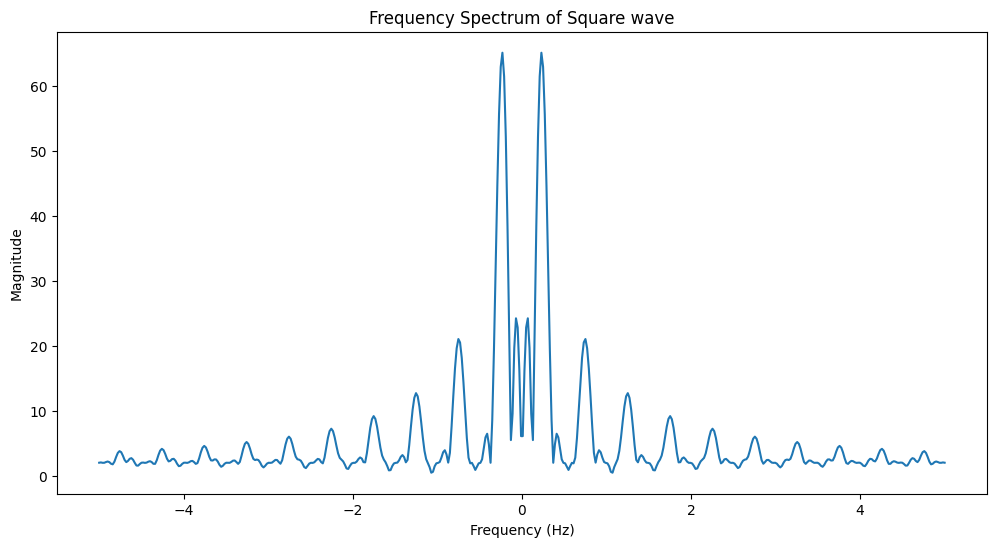
\includegraphics[width=0.8\linewidth]{images/freqSpectrum.png}
        \caption{Frequency spectrum of square signal}
        \label{fig:enter-label}
    \end{figure}  
  \end{frame}
  
  \begin{frame}
    \frametitle{Application of Fourier Transform: \textcolor{yellow}{Filtering}}
    \begin{itemize} [label=$\star$, itemsep=4pt, parsep=0pt, topsep=10pt]
        \item<1-> Filter:  \textbf{\textcolor{red}{Low Pass Filter}}
    \end{itemize}
    \vspace{-10pt}
    \begin{figure}
        \centering
        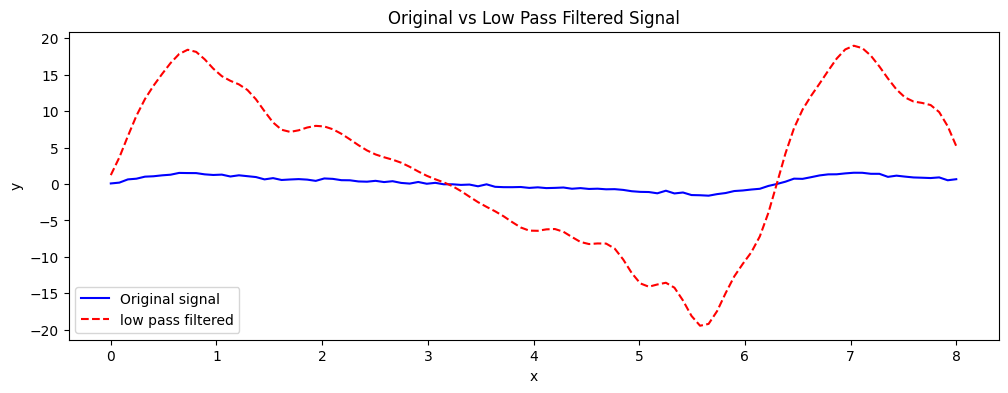
\includegraphics[width=0.8\linewidth,height=0.5\linewidth]{images/lowPassFilter.png}
        \caption{Low pass filtered signal of a noisy signal}
        \label{fig:enter-label}
    \end{figure}
  \end{frame}
  
  \begin{frame}
    \frametitle{Application of Fourier Transform: \textcolor{yellow}{Filtering}}
    \begin{itemize} [label=$\star$, itemsep=4pt, parsep=0pt, topsep=10pt]
        \item<1-> Filter:  \textbf{\textcolor{red}{High Pass Filter}}
    \end{itemize}
    \vspace{-10pt}
    \begin{figure}
        \centering
        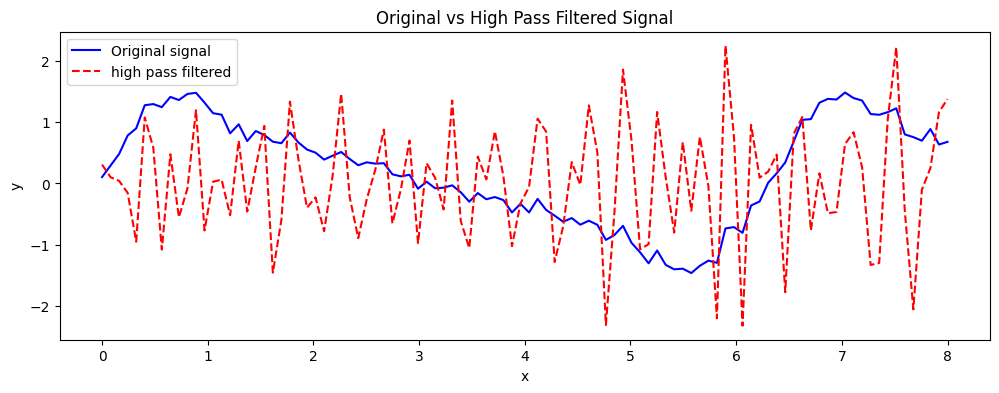
\includegraphics[width=0.8\linewidth,height=0.5\linewidth]{images/highPassFilter.png}
        \caption{High pass filtered signal of a noisy signal}
        \label{fig:enter-label}
    \end{figure}
  \end{frame}
  
  \begin{frame}
    \frametitle{Application of Fourier Transform: \textcolor{yellow}{Filtering}}
    \begin{itemize} [label=$\star$, itemsep=4pt, parsep=0pt, topsep=10pt]
        \item<1-> Filter:  \textbf{\textcolor{red}{Band Pass Filter}}
    \end{itemize}
    \vspace{-10pt}
    \begin{figure}
        \centering
        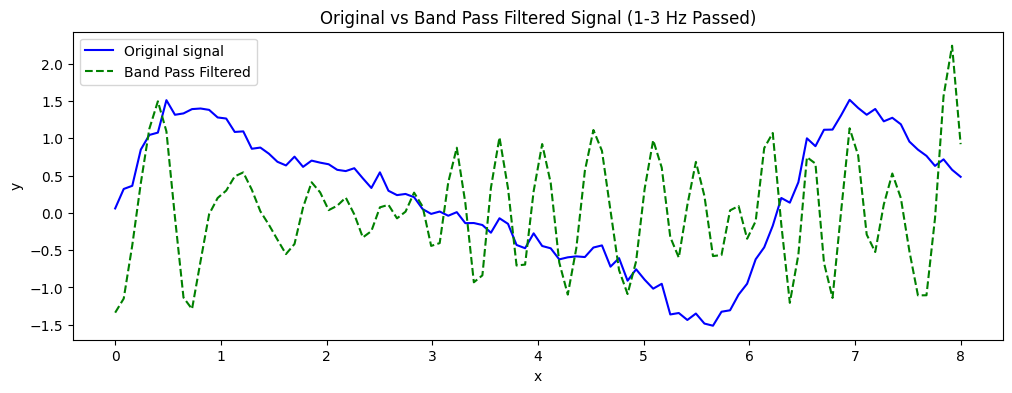
\includegraphics[width=0.8\linewidth,height=0.5\linewidth]{images/bandPassSignal.png}
        \caption{Band pass filtered signal of a noisy signal}
        \label{fig:enter-label}
    \end{figure}
  \end{frame}
  
  \begin{frame}
    \frametitle{Application of Fourier Transform: \textcolor{yellow}{Filtering}}
    \begin{itemize} [label=$\star$, itemsep=4pt, parsep=0pt, topsep=10pt]
        \item<1-> Filter:  \textbf{\textcolor{red}{Band Reject Filter}}
    \end{itemize}
    \vspace{-10pt}
    \begin{figure}
        \centering
        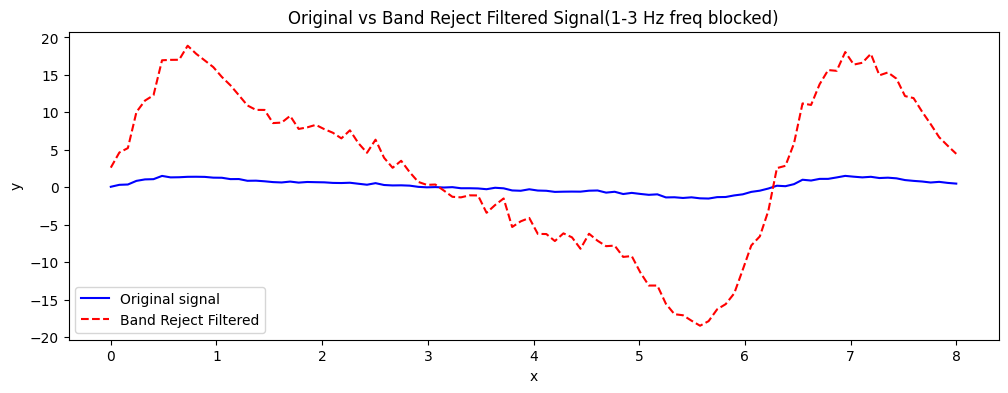
\includegraphics[width=0.8\linewidth,height=0.5\linewidth]{images/bandRejectSignal.png}
        \caption{Band reject filtered signal of a noisy signal}
        \label{fig:enter-label}
    \end{figure}
  \end{frame}
  
  \begin{frame}
    \frametitle{Application of Fourier Transform: \textcolor{yellow}{Image Processing}}
    \begin{itemize}[label=$\star$, itemsep=7pt, parsep=0pt, topsep=10pt]
       \item<1-> \textbf{\textcolor{red}{Frequency Analysis}} 
           \begin{itemize} [label=$\bullet$, itemsep=7pt, parsep=0pt, topsep=10pt]
               \item<2-> FT separates \textcolor{red}{high-frequency} components from \textcolor{red}{low-frequency} components. This helps in analyzing \textcolor{blue}{image characteristics}
           \end{itemize}
    \end{itemize}
    \vspace{10pt}
    \begin{figure}
        \centering
        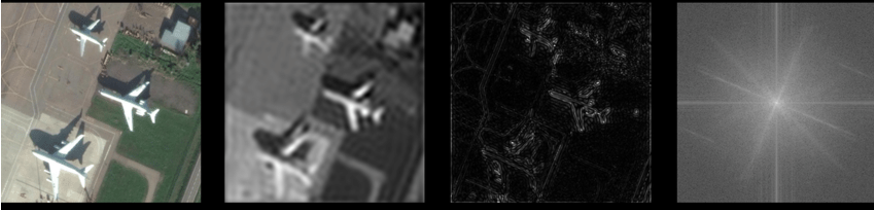
\includegraphics[width = 0.7\textwidth]{images/lowFreqHighFreq.png}
        \caption{From right to left: Original image, Low-frequency components, High frequency components,Fourier transform}
    \end{figure}
    \vfill 
    \tiny \textit{Image source:} \url{https://www.researchgate.net/figure/sualization-of-low-frequency-components-high-frequency-components-and-Fourier-spectrums_fig2_347515196} 
  \end{frame}
  
  \begin{frame}
     \frametitle{Application of Fourier Transform: \textcolor{yellow}{Image Processing}}
     \begin{itemize}[label=$\star$, itemsep=7pt, parsep=0pt, topsep=10pt]
     \item<1-> \textbf{\textcolor{red}{Compression}}
    \end{itemize} 
    \vspace{-10pt}
    \begin{figure}
        \centering
        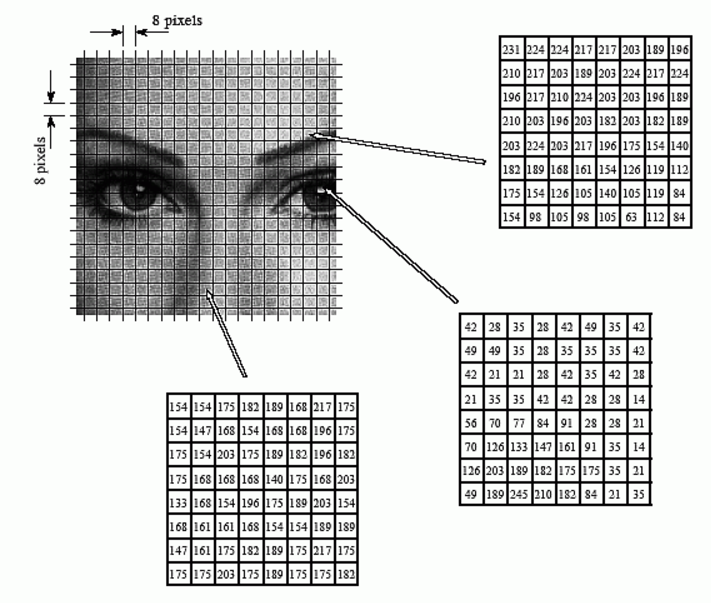
\includegraphics[width=0.5\linewidth]{images/imageCmp2.png}
        \caption{JPEG Transform compression}
        \label{fig:enter-label}
    \end{figure}
    \vfill 
    \tiny \textit{Image source:}
    \url{https://www.dspguide.com/ch27/6.htm}
  \end{frame}
  
  \begin{frame}
    \frametitle{Application of Fourier Transformation: \textcolor{yellow}{Image Processing}}
    \begin{itemize} [label=$\star$, itemsep=4pt, parsep=0pt, topsep=10pt]
        \item<1-> \textbf{\textcolor{red}{Image Reconstruction}}
    \end{itemize}
    \vspace{5pt}
    \hspace{20pt}
    \begin{tikzpicture}
          % Node for the first figure
          \node<1->[anchor=center] (fig1) at (0,1) {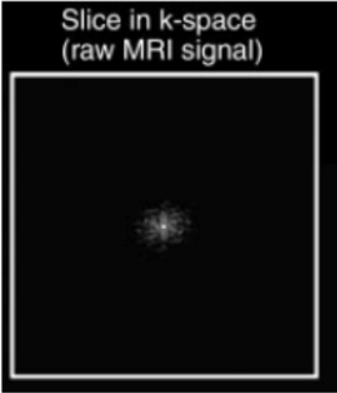
\includegraphics[width=4cm,height=4cm]{images/kSpaceSignal.png}};
  
          \draw<2->[->, thick, red] (fig1.east) -- ++(2, 0)
               node[midway, above=5pt] {\tiny Inverse Fourier Transform};
          
          % Node for the second figure
          \node<3->[anchor=center] (fig2) at (7, 1) {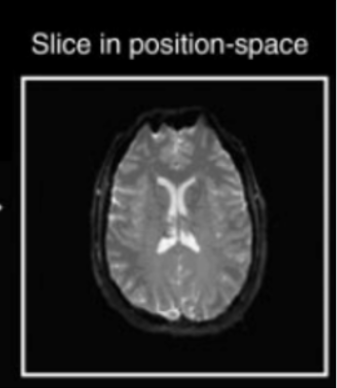
\includegraphics[width=4cm,height=4cm]{images/positionSpaceSignal.png}};
          
    \end{tikzpicture}
     \begin{center}
       \scriptsize \textcolor{blue}{Figure:} Fourier transform in \textcolor{red}{Medical Imaging}
    \end{center}
    \vfill 
    \tiny \textit{Image source:}
    \url{https://www.researchgate.net/figure/A-a-Fourier-transform-is-applied-to-the-q-space-images-to-reconstruct-the-image-in-the_fig12_281047295}
  \end{frame}
  
  
  \begin{frame}
    \frametitle{Application of Fourier Transformation: \textcolor{yellow}{Image Processing}}
    \begin{itemize} [label=$\star$, itemsep=4pt, parsep=0pt, topsep=10pt]
        \item<1-> \textbf{\textcolor{red}{Image Reconstruction}}
    \end{itemize}
    \vspace{-5pt}
    \hspace{20pt}
    \begin{tikzpicture}
          % Node for the first figure
          \node<1->[anchor=center] (fig1) at (0,1) {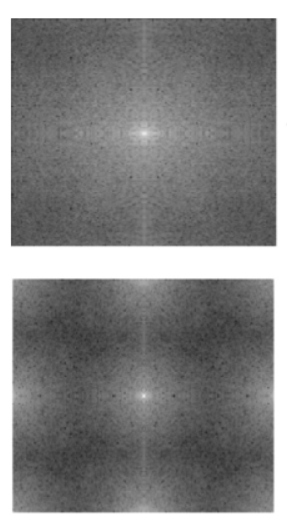
\includegraphics[width=3cm,height=5cm]{images/mri1.png}};
          
          % Node for the second figure
          \node<3->[anchor=center] (fig2) at (5.5, 1) {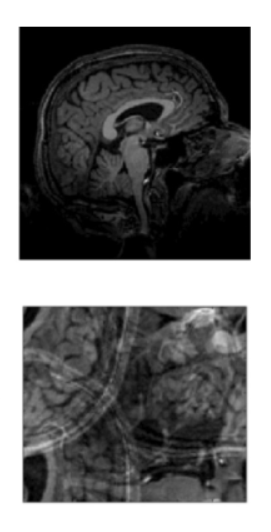
\includegraphics[width=3cm,height=5cm]{images/mri2.png}};
  
          % Arrow from middle of fig1 to fig2
          \draw<2->[->, thick, red] (fig1.east) -- (fig2.west)
               node[midway, above=5pt] {\tiny 2D Inverse Fourier Transform};
          
          % Arrow from middle of fig1 to fig2
          \draw<2->[->, thick, red] (fig1.east) -- (fig2.west)
               node[midway, below=5pt] {\tiny Inverse Fourier Transform};
          
    \end{tikzpicture}
     \begin{center}
       \scriptsize \textcolor{blue}{Figure:} Fourier Reconstruction in \textcolor{red}{MRI}
    \end{center}
    \vfill 
    \tiny \textit{Image source:}
    \url{https://link.springer.com/chapter/10.1007/978-3-030-30511-6_9}
  \end{frame}
  
  \begin{frame}
    \frametitle{Application of Fourier Transformation: \textcolor{yellow}{Audio Processing}}
    \begin{itemize} [label=$\star$, itemsep=4pt, parsep=0pt, topsep=10pt]
        \item<1-> \textbf{\textcolor{red}{Removing Noise} } 
    \end{itemize}
    \vspace{5pt}
    \hspace{25pt}
    \begin{tikzpicture}
          % Node for the first figure
          \node<1->[anchor=center] (fig1) at (0, 0) {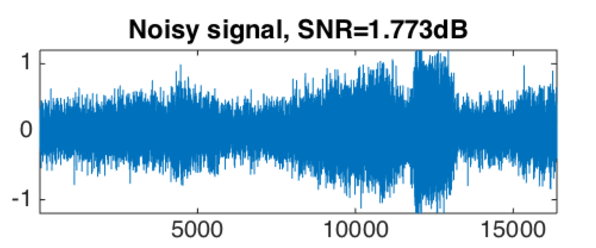
\includegraphics[width=4cm,height=3cm]{images/noisySignal.png}};
  
          \draw<2->[->, thick, red] (fig1.east) -- ++(2, 0)
               node[midway, above=5pt] {\tiny Fourier Transform};
          
          % Node for the second figure
          \node<3->[anchor=center] (fig2) at (7, 0) {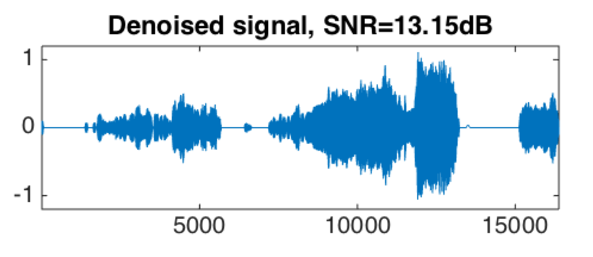
\includegraphics[width=4cm,height=3cm]{images/denoisedAudio.png}};
          
    \end{tikzpicture}
     \begin{center}
       \scriptsize \textcolor{blue}{Figure:} Comparison of \textcolor{red}{Noisy} and \textcolor{red}{Denoised} Signal Using Fourier Transform
    \end{center}
    \vfill 
    \tiny \textit{Image source:}
    \url{https://www.numerical-tours.com/matlab/audio_1_processing/}  
  \end{frame}
  
  \begin{frame}
    \frametitle{Application of Fourier Transformation: \textcolor{yellow}{Audio Processing}}
    \begin{itemize} [label=$\star$, itemsep=7pt, parsep=0pt, topsep=10pt]
        \item<1-> Equalization
        \item <2-> Pitch shifting and time stretching
        \item <3-> Sound synthesis
        \item <4-> Audio effects
        \item <5-> Real time audio processing:
            \begin{itemize}[label=$\bullet$, itemsep=7pt, parsep=0pt, topsep=10pt]
                \item<6-> Live Sound Enhancement
                \item<7-> Interactive Audio
            \end{itemize}
        \item <8-> Audio Fingerprinting
    \end{itemize} 
  \end{frame}
\end{document}
